\documentclass[a4paper]{article}

\usepackage[english]{babel}
\usepackage[utf8x]{inputenc}
\usepackage{amsmath}
\usepackage{graphicx}
\usepackage[colorinlistoftodos]{todonotes}
\usepackage{subfig}
\usepackage{float}


%_____________________________________________________________________________________
% THIS SOME THING THAT WILL GET OUR FIGURES IN THE RIGHT PLACE TAKEN FROM THE INTERNET ON THE WEBPAGE; http://mintaka.sdsu.edu/GF/bibliog/latex/floats.html

%%% START %%%
% Alter some LaTeX defaults for better treatment of figures:
    % See p.105 of "TeX Unbound" for suggested values.
    % See pp. 199-200 of Lamport's "LaTeX" book for details.
    %   General parameters, for ALL pages:
    \renewcommand{\topfraction}{0.9}	% max fraction of floats at top
    \renewcommand{\bottomfraction}{0.8}	% max fraction of floats at bottom
    %   Parameters for TEXT pages (not float pages):
    \setcounter{topnumber}{2}
    \setcounter{bottomnumber}{2}
    \setcounter{totalnumber}{4}     % 2 may work better
    \setcounter{dbltopnumber}{2}    % for 2-column pages
    \renewcommand{\dbltopfraction}{0.9}	% fit big float above 2-col. text
    \renewcommand{\textfraction}{0.07}	% allow minimal text w. figs
    %   Parameters for FLOAT pages (not text pages):
    \renewcommand{\floatpagefraction}{0.7}	% require fuller float pages
	% N.B.: floatpagefraction MUST be less than topfraction !!
    \renewcommand{\dblfloatpagefraction}{0.7}	% require fuller float pages

	% remember to use [htp] or [htpb] for placement
    
%%% END %%%
%_____________________________________________________________________________________

% NEEDED FOR THE REFERENCE
 %_______SOURCE; 

% START
\usepackage{hyperref}
% END


% NEEDED FOR SOURCE CODE (JAVA) TO FUNCTION NICELY
% SOURCE; http://stackoverflow.com/questions/3175105/how-to-insert-code-into-a-latex-doc
%START
\usepackage{listings}
\usepackage{color}
\definecolor{dkgreen}{rgb}{0,0.6,0}
\definecolor{gray}{rgb}{0.5,0.5,0.5}
\definecolor{mauve}{rgb}{0.58,0,0.82}

\lstset{frame=tb,
  language=Java,
  aboveskip=3mm,
  belowskip=3mm,
  showstringspaces=false,
  columns=flexible,
  basicstyle={\small\ttfamily},
  numbers=none,
  numberstyle=\tiny\color{gray},
  keywordstyle=\color{blue},
  commentstyle=\color{dkgreen},
  stringstyle=\color{mauve},
  breaklines=true,
  breakatwhitespace=true,
  tabsize=3
}
%END





\title{Design and Control of a Lego Unicycle}
\author{Group B: Johan Kellerth Fredlund | Koshin Aliabase\\ Santiago Castro Chans | Sadik Kenan Sulejmanovic}

\begin{document}
\maketitle

\clearpage
\begin{abstract}
The goal of this project was to design a controller that could balance a unicycle in the medial direction, using a ground wheel, and in the lateral direction using an inertia wheel. Due to the complexity of the problem the control of the lateral direction was focused on. The model was determined using Newton's laws and the linearization around the origin was controlled using LQR. Using the program LeJos written in java the controller was implemented. The simulink model was stable but the real process turned out to be unstable. It was unstable because the sensors were not accurate enough and the micro controller was not fast enough for the many nested classes in LeJos. Since the measurements took too long to be received by the micro controller the system could not be stable.
\end{abstract}
\clearpage
\tableofcontents

\section{Author's note}

The project has been a great learning experience for us. We have learned about Lagrangian equations, system identification, the physics of a pendulum, desired variables for optimal control and much more. We have dedicated our souls for this project for 6 weeks and have had a lot of fun while doing it. The project was very comprehensive which was challenging and caused much dedication among us to make it work. 

We would like to thank our supervisor Olof Troeng, who helped us with problems when we were stuck, Anders Nilsson who gave us access to a computer where we could download LeJos, Anders Robertsson who also helped by loaning us a book about the inertia wheel, and Sergej Rumjantsev who spent a whole day helping us build the inertia wheel.
\clearpage

\section{Introduction}

We are designing a unicycle made by lego with an integrated inertia wheel to keep the lateral balance. The project therefore consists of two problems. To stabilize the unicycle in the medial direction by designing a controller for the ground wheel, and to stabilize it in the lateral direction by applying a reaction wheel connected to the top of the unicycle.

\section{Construction}

	\subsection{Ev3}
	The EV3 is the third generation of Lego Mindstorms platforms, the specification of this platform can be seen in the table \ref{table:spec_ev3}. Furthermore some options for programming platforms are listed in the table \ref{table:prog_platforms_ev3}. Lastly can a picture of the EV3 also be seen in figure \ref{fig:ev3_platform_picture}
	
	 \begin{table}[h]
		\center
		\begin{tabular}{|c |c|}
			\hline
			 Processor &  ARM9   \\ 
			\hline
			OS   & Linux- based  \\ 
			\hline
			Sensor ports & 4 , analog, digital (up to 460.8 Kbit/sec)  \\
	        		\hline
			Motor port & 4, with encoders \\
			\hline
			SD- card & Micro SD- Card Reader, (up to 32 GB)   \\
			\hline
		\end{tabular}
		\caption{Specifications for the EV3 platform found at \cite{EV3spec}.}
		\label{table:spec_ev3}
	\end{table}
	
	 \begin{table}[h]
		\center
		\begin{tabular}{|c|}
			\hline
			Programing platforms   \\ 
			\hline
			Lejos (extension of JAVA)  \\ 
			\hline
			RobotC (similar to C) \\
	        		\hline
			NCX (similar to C )\\
			\hline
		\end{tabular}
		\caption{Some of the optional programing platforms for the EV3.}
		\label{table:prog_platforms_ev3}
	\end{table}
	
	
	
		\begin{figure}[h]
		\centering
		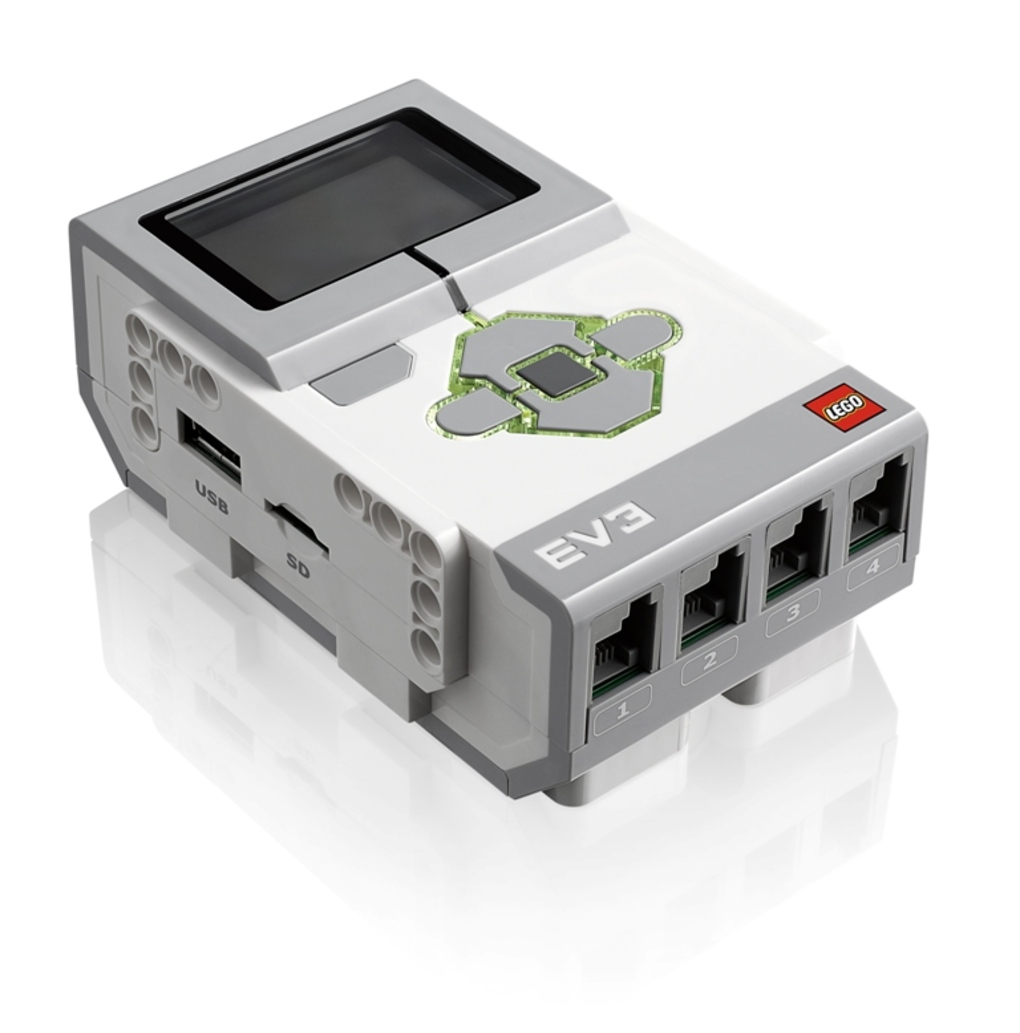
\includegraphics[width=0.2\textwidth,height=0.2\textheight]{ev3_platform}
		\caption{Shows how the hardware platform EV3 looks like which was used in the project.}
		\label{fig:ev3_platform_picture}
	\end{figure}
	
	
	
	
    \subsection{Sensors}
    	\subsubsection{HighTechinic Gyro Sensor}
        The Gyro sensor gives the rate of change in x, y and z orientation in radians per second. More specified details about the sensor can be seen in the table \ref{table:Gyro_sensor}. The first row shows how long time it takes for our program to fetch a sample, second row shows how accurate the sensor is given by specification by the manufacturer and the last line shows the update time of the sensor also given by the manufacturer. 
\\In nature all gyroscopes has a drift and offset, both are unwanted. The drift means that the rate of change will increase with time even though the sensor is stationary as can been observed in the figure \ref{fig:Gyro_offsets_refresh_times}. Secondly the offset is the property that give a constant value although the sensor is stationary. How we dealt with these problems will be explained in later sections. Lastly can we see the gyro sensor in figure \ref{fig:NXT_Gyro_Sensor}.  
        
        
        % THE TABLE DESCRIBING THE PROP. of the gyro sensor
        \begin{table}[h]
		\center
		\begin{tabular}{|c |c|}
			\hline
			 Refresh time in program & 10 ms (average)   \\ 
			\hline
			Accuracy &  $\pm 1$ degree \cite{NXT_Gyro_Sensor} \\ 
			\hline
			Update of value & 300 times / second  \cite{NXT_Gyro_Sensor} \\
	        		\hline
		\end{tabular}
		\caption{Specifications for the gyro under the name NXT Gyro Sensor (NGY1044).}
		\label{table:Gyro_sensor}
	\end{table}


	\begin{figure}[h]
		\centering
		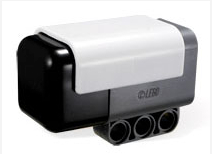
\includegraphics[width=0.3\textwidth]{NXT_Gyro_Sensor}
		\caption{Shows the gyro sensor which was used in the project.}
		\label{fig:NXT_Gyro_Sensor}
	\end{figure}
	
	\begin{figure}[h]
		\centering
		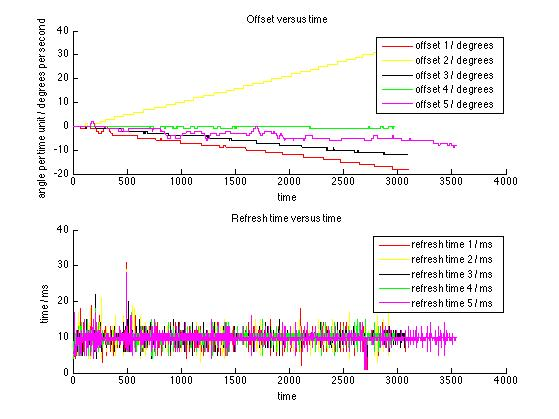
\includegraphics[width=1.3\textwidth]{plot_gyro_test_final_20150107}
		\caption{Shows the gyro sensor's offsets and refresh times when beeing stationary.}
		\label{fig:Gyro_offsets_refresh_times}
	\end{figure}
	
	\newpage
        
        
        \subsubsection{HighTechinic Accelerometer Sensor}
        
The accelerometer measure acceleration in x, y and z direction relative to the sensors specified directions given by the manufacturer. The specifications of the accelerometer can be seen in the table \ref{table:Acce_sensor} which shows the the time for it to give a sample to our program respectively number of times the sensor can update a value. On the other hand this sensor also comes with unwanted properties which is that the value is (very) noise however when it is not noise it gives reasonable good data. We can also see how this sensor looks like in the figure \ref{fig:NXT_Acce_Sensor} and the refresh time for a longer of time can be seen in the figure \ref{fig:plot_acce_refresh_time}
         % THE TABLE DESCRIBING THE PROP. of the Acce sensor
         \begin{table}[h]
		\center
		\begin{tabular}{|c |c|}
			\hline
			 Refresh time in program & 20 ms (average)   \\ 
			\hline
			Update of value &  100 times / second \cite{NXT_Acce} \\ 
			\hline
		\end{tabular}
		\caption{Specifications for the accelerometer under the name NXT Acceleration (NAC1040).}
		\label{table:Acce_sensor}
	\end{table}
	
	\begin{figure}[h]
		\centering
		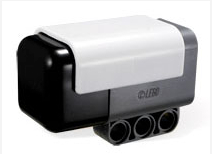
\includegraphics[width=0.3\textwidth]{NXT_Gyro_Sensor}
		\caption{Shows the accelerometer sensor which was used in the project.}
		\label{fig:NXT_Acce_Sensor}
	\end{figure}
	
	\begin{figure}[h]
		\centering
		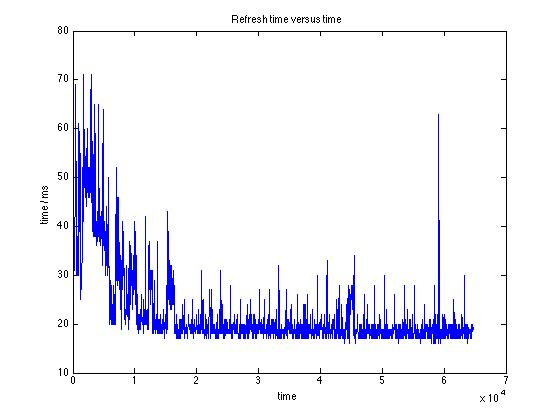
\includegraphics[width=1.3\textwidth]{plot_acce_refresh_time_20150107}
		\caption{Shows the accelerometer sensor refresh time.}
		\label{fig:plot_acce_refresh_time}
	\end{figure}
	
	
         
        
        
        \subsubsection{AbsoluteIMU-ACG}
        The AbsoluteIMU-ACG can gives gyro, accelerometer and compass data but in this project we are only interested in the gyro and the accelerometer therefor we will only discuss those measurements. As discussed previously gives the gyro part the rate of change in x,y and z. The accelerometer part measures the gravity in the x,y and z direction. The interesting part of this sensor is the refresh time versus the previous sensors and the update time can be seen in the figure \ref{fig:plot_IMU_sensor_sensitivity_0}. With this sensor one can also choose to have a smoothing filter for the accelerometer part of the IMU, downside is that this will increase the refresh time of the sensor. Therefor we did two measurements, one with sensitivity 0 and one with sensitivity 4 (figure \ref{fig:plot_IMU_sensor_sensitivity_4}). 
        
        \begin{figure}[h]
		\centering
		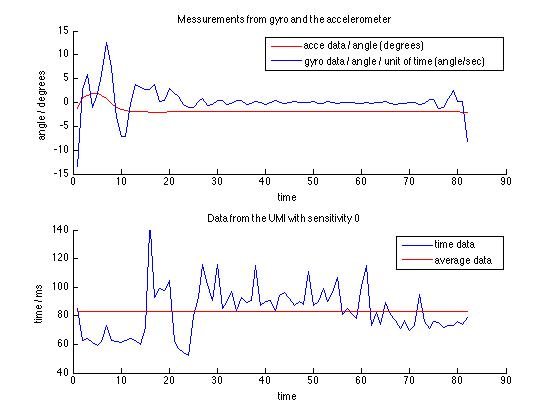
\includegraphics[width=1.3\textwidth]{plot_data_UMI_sen_0_20150103}
		\caption{Shows the important properties of the IMU sensor with sensitivity 0.}
		\label{fig:plot_IMU_sensor_sensitivity_0}
	\end{figure}
	
	      \begin{figure}[h]
		\centering
		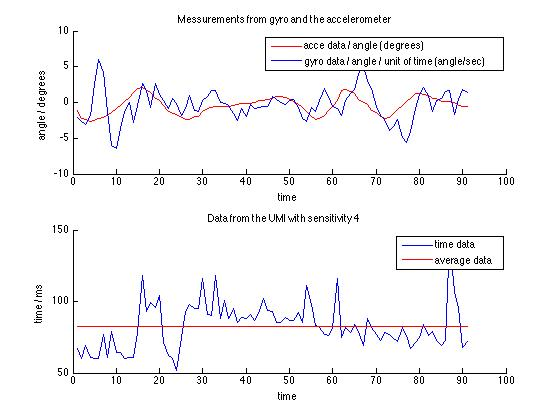
\includegraphics[width=1.3\textwidth]{plot_data_UMI_sen_4_20150107}
		\caption{Shows the important properties of the IMU sensor with sensitivity 4.}
		\label{fig:plot_IMU_sensor_sensitivity_4}
	\end{figure}
	
	
	\begin{table}[h]
		\center
		\begin{tabular}{|c |c|}
			\hline
			 Refresh time in program &  83 ms (average)   \\ 
			\hline
			Update of value &  100 times / second  \cite{IMU_sensor} \\ 
			\hline
		\end{tabular}
		\caption{Specifications for the IMU-ACG sensor.}
		\label{table:IMU_sensor}
	\end{table}
	
        
        
    \newpage 
    \subsection{Reaction wheel}
    
    The reaction wheel modeling is explained in the section \ref{sec:Modeling} and some conclusion can be drawn from that. In this section we will bring up what those conclusion became in reality. Because we want as much weight as possible in the outer ring so nuts screwed in the material was the obvious choice. The choice of material was between plastic and wood, because of the nature of time and availability of personal it became wood. Plastic was preferable wood would also make it work. Due to the heavier weight of wood due to its nature it became a problem but was solved with making circles in the circle of wood so the most of the weight was taken out but leave enough for the circle not to crack under pressure of acceleration. The end product of the reaction wheel can be seen in the figure \ref{fig:reaction_wheel_end_product} while the dimensions is shown in the table \ref{table:spec_reaction_wheel}. Meanwhile the design of the initial reaction wheel be seen in the figure \ref{fig:reaction_wheel_initial_design}. Thirdly is wort mentioning that the wholes at the end of the circle in figure \ref{fig:reaction_wheel_initial_design} is for the nuts to go in and the cross in the middle is for the attachment to the axis going to the EV3 Large Servo Motor. More on this topic under the section \ref{sec:Attachment_reaction_wheel_EV3_Motor}
    
    
       \begin{figure}[h]
		\centering
		\includegraphics[width=0.5\textwidth,height=0.5\textwidth]{reaction_wheel_initial_design}
		\caption{Shows the initial design for the reaction wheel.}
		\label{fig:reaction_wheel_initial_design}
	\end{figure}
	
	
	\begin{table}[h]
		\center
		\begin{tabular}{|c |c|}
			\hline
			Diameter & 30 cm    \\ 
			\hline
			Thickness & 8 mm  \\ 
			\hline
		\end{tabular}
		\caption{Shows the dimensions of the end product of the reaction wheel.}
		\label{table:spec_reaction_wheel}
	\end{table}
	
      \begin{figure}[h]
		\centering
		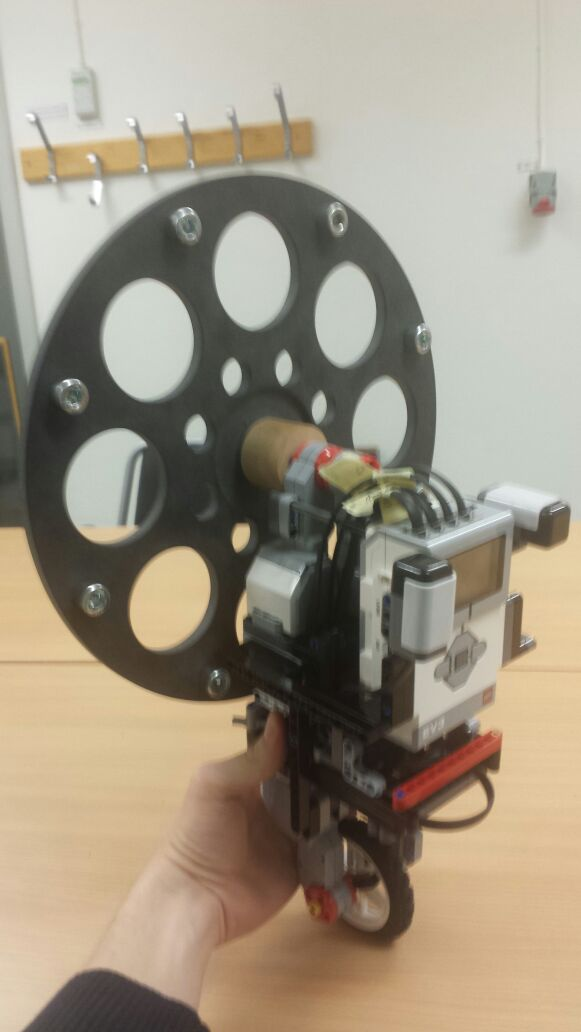
\includegraphics[width=0.7\textwidth,height=0.7\textwidth]{reaction_wheel_endproduct_picture}
		\caption{Shows the end product of the reaction wheel with the whole prototype at one stage.}
		\label{fig:reaction_wheel_end_product}
	\end{figure}
    
    
    
    
    
    
    
    
    \newpage
 \subsubsection{Attachment between the reaction wheel and EV3 Large Motor } 
 \label{sec:Attachment_reaction_wheel_EV3_Motor}
 
 Due to the attachment of the sensors on the current prototype we build in one small circular block to the reaction wheel which also had wholes matching the attachment directly to the EV3 Motor attachment. The specific attachment pattern is shown in figure \ref{fig:pattern_EV3_attachment}. By using that specific pattern we achieved more stability of the reaction wheel but still there were problems with leaning of the reaction wheel relative to the full scale prototype. We also experienced wobbling of the reaction wheel when it was set to use. Therefore we rebuild the reaction wheel once more relative to the initial design with one more circular block on the other side of the reaction wheel which meant that we now had two circular blocks coming out from the reaction wheel at both ends. The prototype holding up the reaction wheel was also rebuild due to rebuilding of the reaction wheel, more on rebuilding of the full prototype can be seen in section \ref{sec:Prototypes}. Thus in the end leading to a full stable reaction wheel relative to the full scale prototype. The end attachment of the reaction wheel is shown in figure \ref{fig:reaction_wheel_attachment_end_product}
 
    \begin{figure}[h]
		\centering
		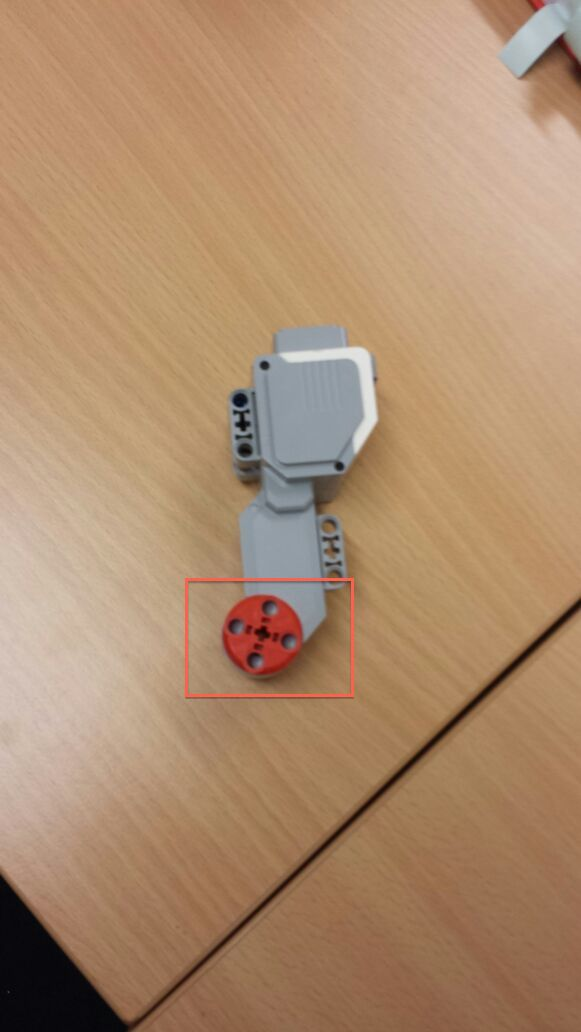
\includegraphics[width=0.3\textwidth]{attachment_pattern_EV3_Large_Motor}
		\caption{The red rectangle specifies the attachment pattern on the EV3 motor.}
		\label{fig:pattern_EV3_attachment}
	\end{figure}


	
	    \begin{figure}[h]
		\centering
		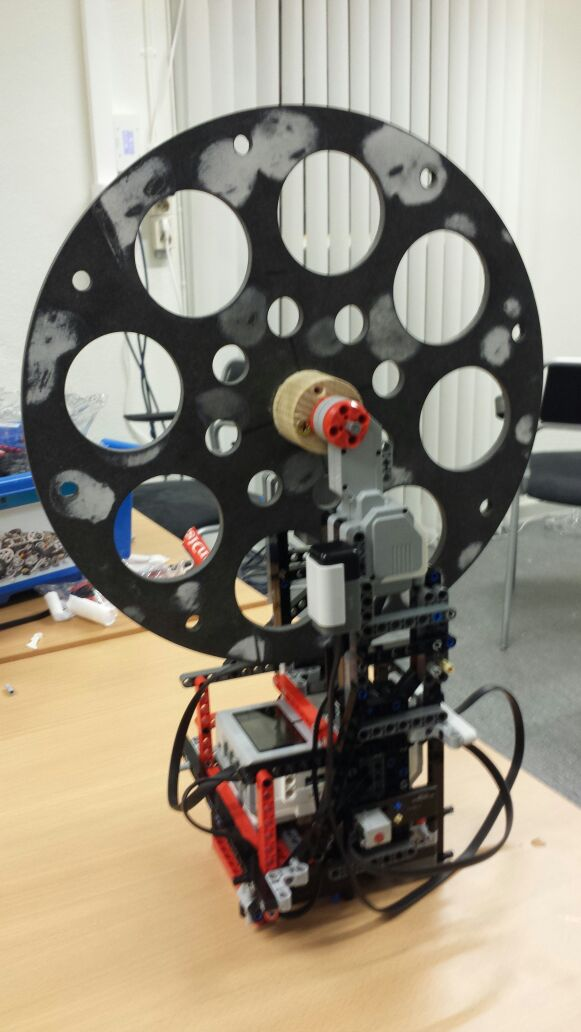
\includegraphics[width=0.5\textwidth,height=0.5\textheight]{reaction_wheel_attachment_end_product}
		\caption{Shown the end product of the attaching of the reaction wheel with the two engines.}
		\label{fig:reaction_wheel_attachment_end_product}
	\end{figure}
	
 
    \newpage
    \subsection{Motors}
    	\subsubsection{EV3 Large Servo Motor}
	\label{sec:EV3 Large Servo Motor}
	This is one of the strongest motors there is for LEGO and the specifications for this motor can be seen in the table 	  \ref{table:EV3_Large_servo_motor}. One experiment was done to get the connection between the torque and the power which is the parameter that control the PWM that goes to the motor. The power goes from -100 to 100. The result can be seen in the figure \ref{fig:plot_power_torque}.
    
 
       \begin{figure}[h]
		\centering
		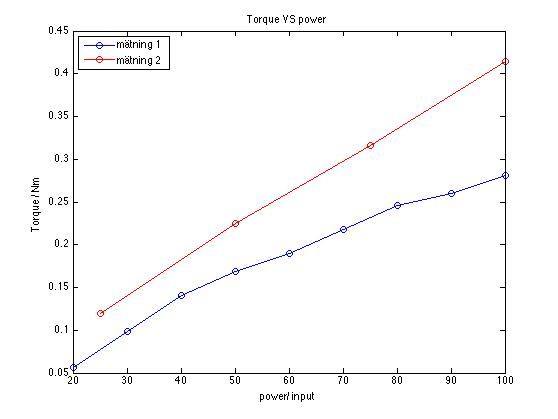
\includegraphics[width=1.3\textwidth]{plot_torque_versus_power_20151207}
		\caption{Shows the relation between the power and the torque of the motor.}
		\label{fig:plot_power_torque}
	\end{figure}
	
	\begin{table}[h]
		\center
		\begin{tabular}{|c |c|}
			\hline
			 RPM &  160 - 170  \cite{Ev3_Large_Servo_Motor}  \\ 
			\hline
			Running torque &  20 N/cm \cite{Ev3_Large_Servo_Motor}  \\ 
			\hline
			Stall torque  &  40 N/cm  \cite{Ev3_Large_Servo_Motor}  \\
			\hline
		\end{tabular}
		\caption{Specifications for the EV3 large motor server.}
		\label{table:EV3_Large_servo_motor}
	\end{table}
	
	
    
    \newpage
    \subsection{Prototypes}
    \label{sec:Prototypes}
In this section we will bring up the limitations of the physical construction of the lego segway and bring up some key limitations of the model as well. \\The most critical limitations is the building blocks of Lego because of some key concepts. The first being that the attachment pieces which holds the lego blocks together are not the most stable one which means that is you put two blocks together you can not expect that the blocks are held together while have some stress on them. They will fold not all the way by enough for the prototype to experience wobbles when the reaction wheel starts to accelerate and move around. This problem was experienced with great signification in the three first prototypes but the last one held it out pretty well considering that the system was made in lego. 

The second limitation is availability of the connection points on the EV3, there are some but could be more of them. From a building perspective this set great boundaries on how you might build your prototype hence the four prototypes. Each of them had strengths and weaknesses which is brought up in the table \ref{table:prototype_properties}. The possible options that the different categories can be are shown in the table \ref{table:def_prototypes}, these options are taken up to give a hint of how the different prototypes act when used and are therefore not scientific in a since that you can measure them. 

 
    
    
 
    \begin{figure}[h]
	\subfloat[]{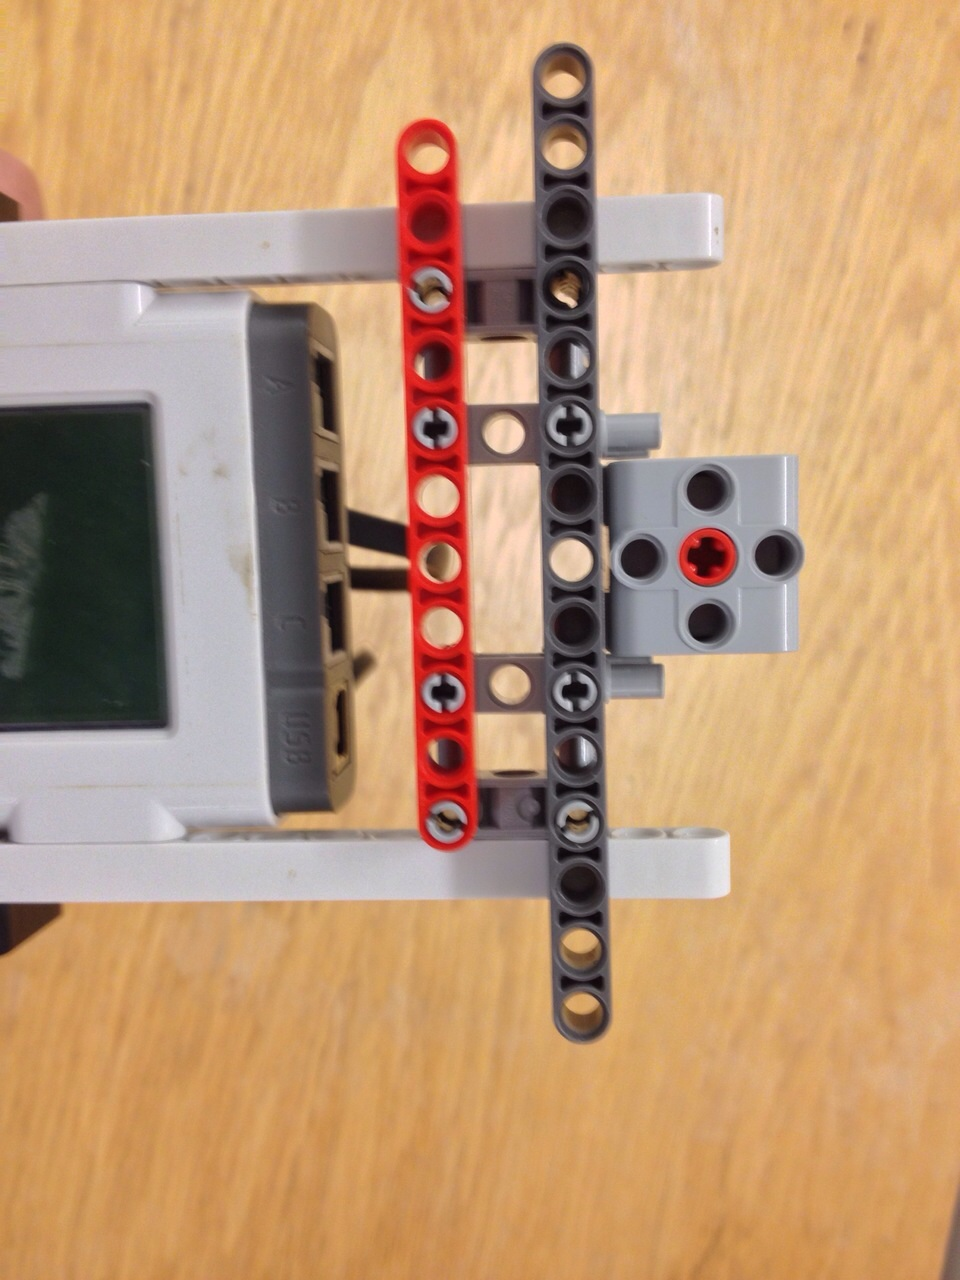
\includegraphics[width=0.3\textwidth,height=0.2\textheight]{prototype_1_a}} 
	\subfloat[]{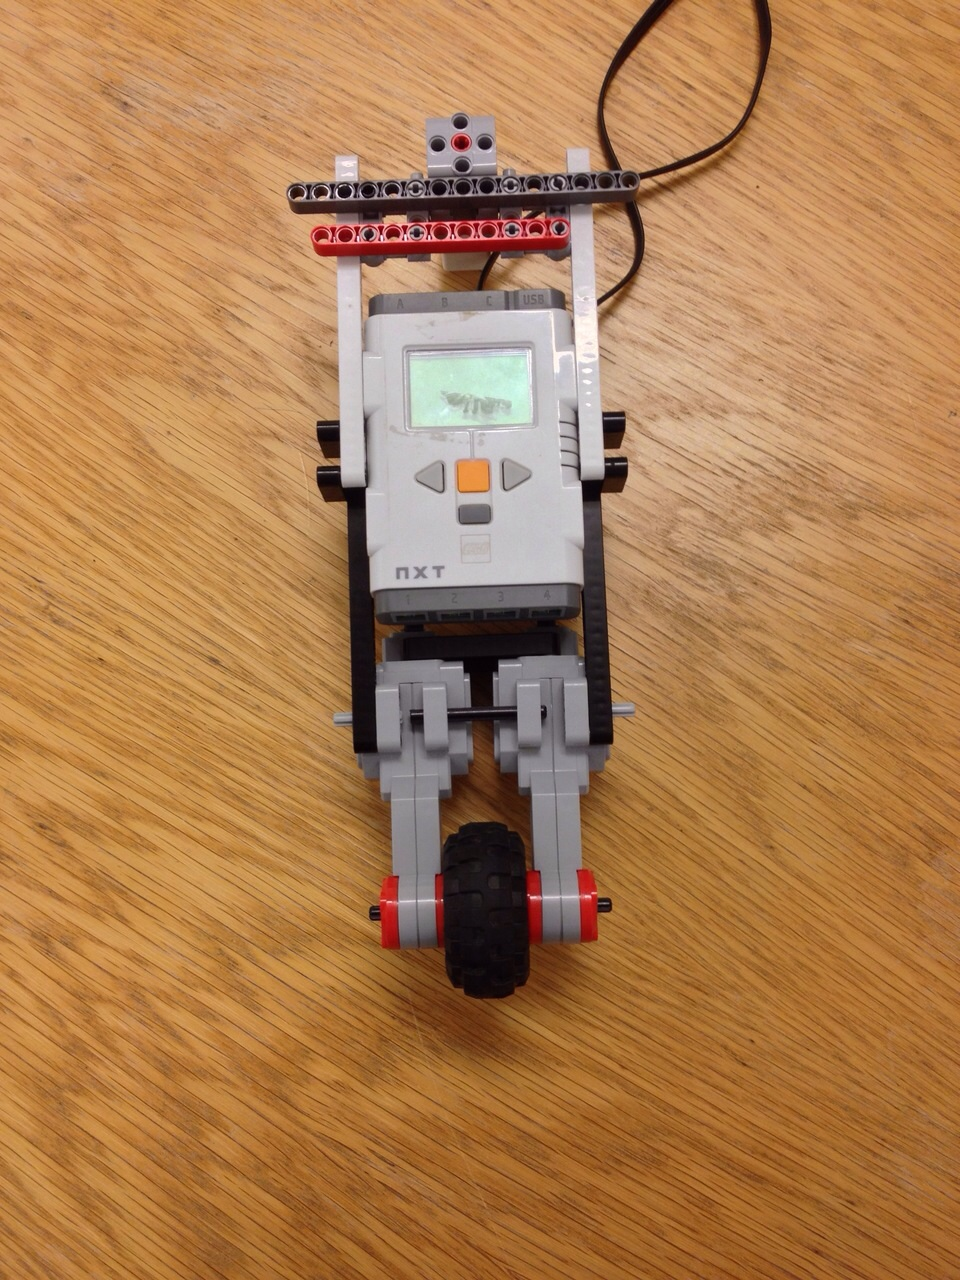
\includegraphics[width=0.3\textwidth,height=0.2\textheight]{prototype_1_b}} 
	\subfloat[]{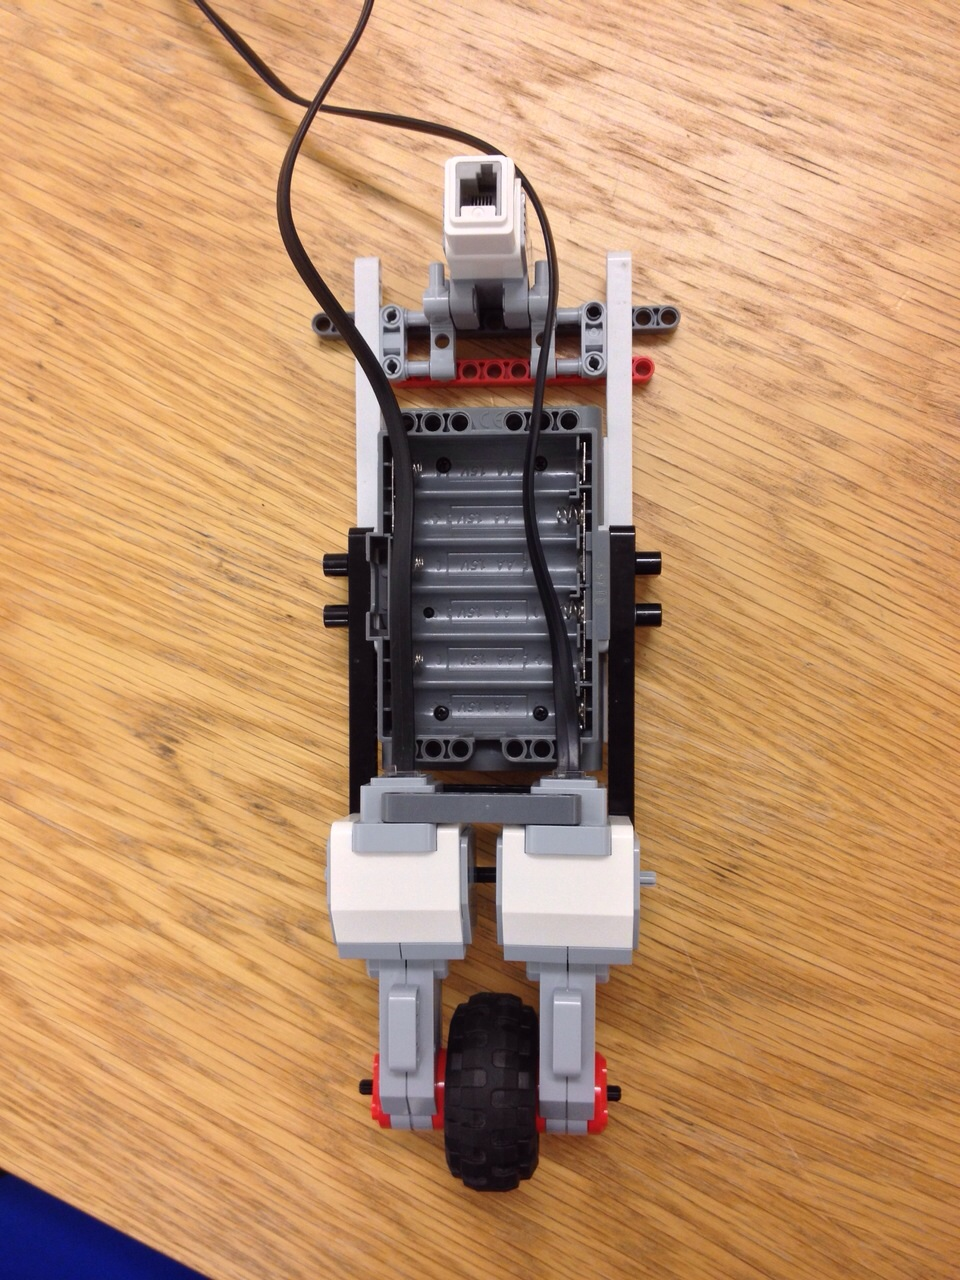
\includegraphics[width=0.3\textwidth,height=0.2\textheight]{prototype_1_c}}  \\
	\subfloat[]{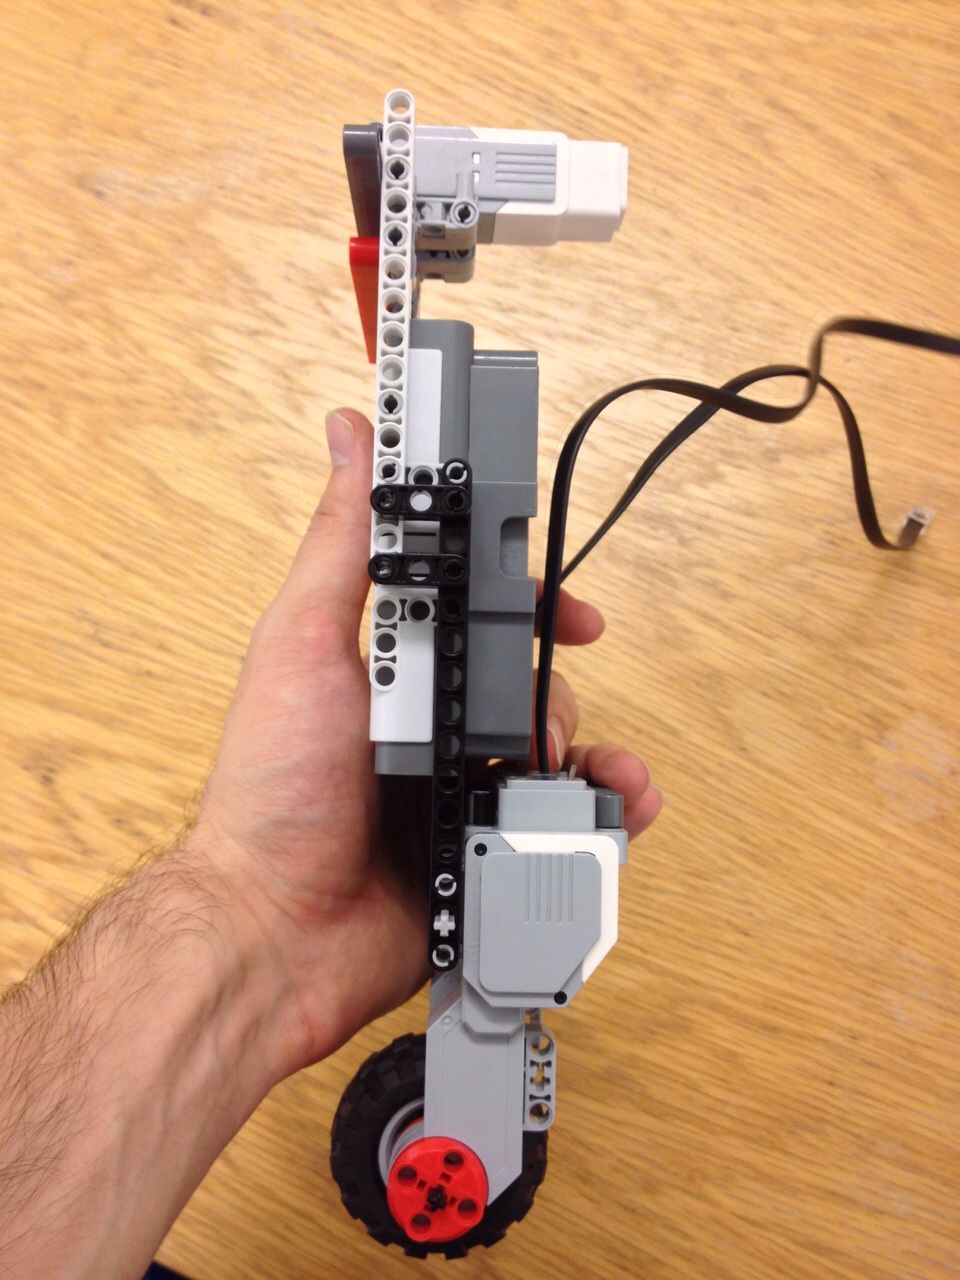
\includegraphics[width=0.3\textwidth,height=0.2\textheight]{prototype_1_d}} 
	\subfloat[]{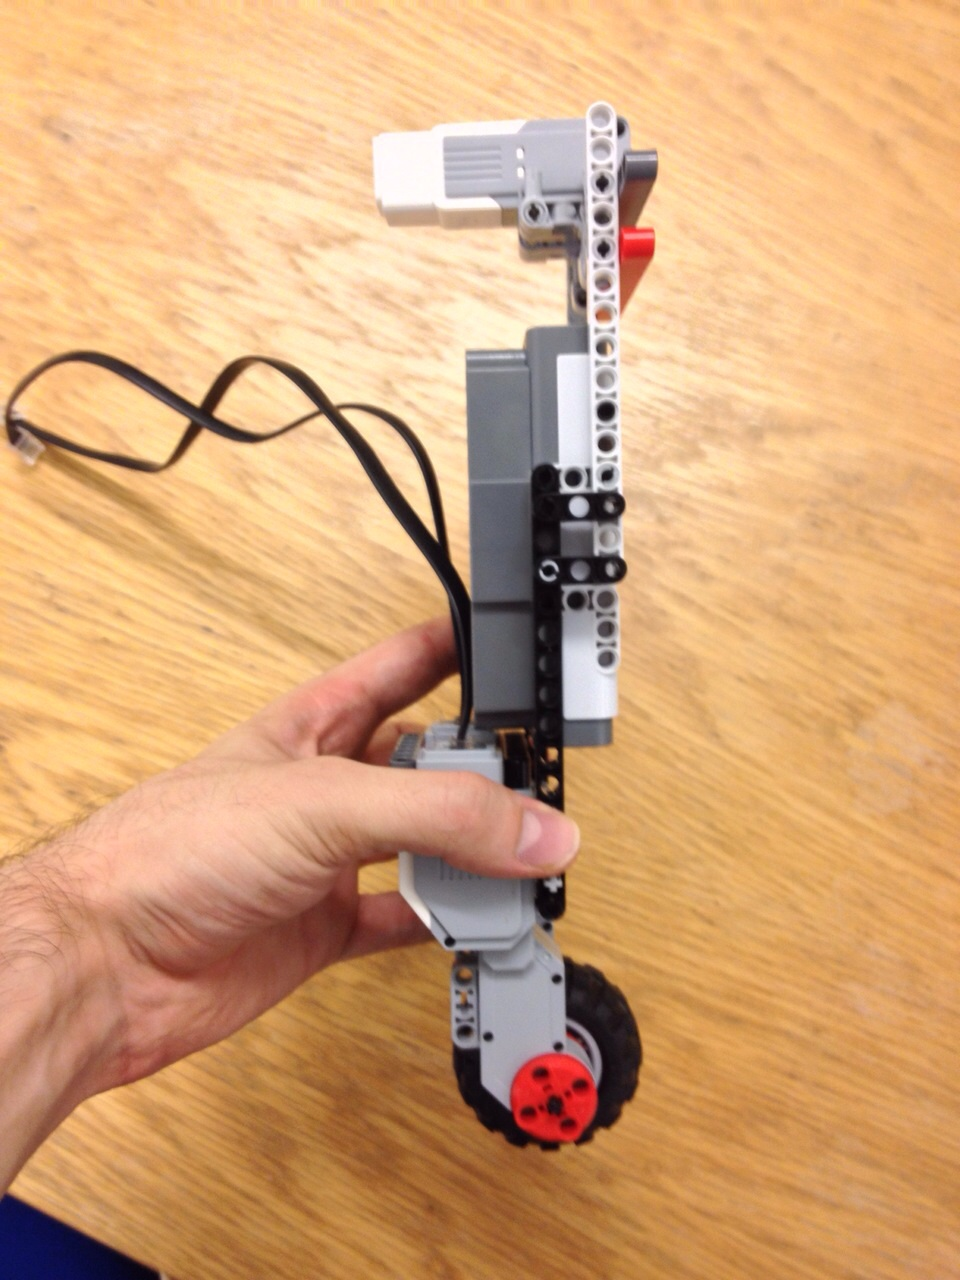
\includegraphics[width=0.3\textwidth,height=0.2\textheight]{prototype_1_e}} 
	\subfloat[]{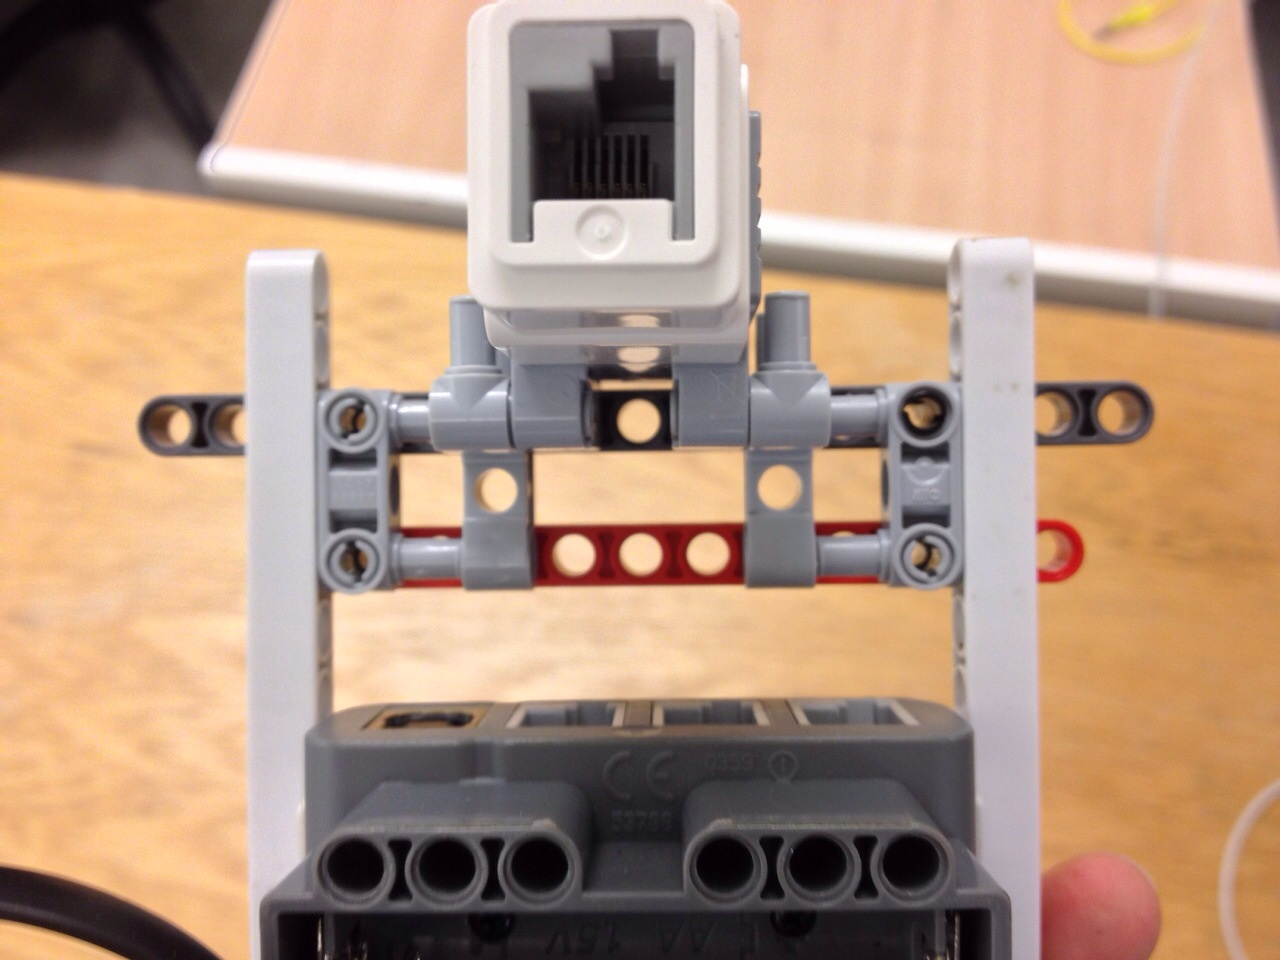
\includegraphics[width=0.3\textwidth,height=0.2\textheight]{prototype_1_f}}
	\caption{Shows the first prototype from different angles.}
    \end{figure}
    
    \begin{table}[h]
		\begin{tabular}{|c |c| |c|  |c|  |c|  }
			\hline
			Categories & p1 & p2 & p3 & p4	\\
			\hline
			 Handle stress due to reaction wheel  & - & falling apart & bad &  good \\ 
			\hline
			Stationary movement &  - &  forward & weak forward & stationary \\ 
			\hline
			Gravidation centre  &  middle  & high & high & low \\
			\hline
			Reaction wheel torn out  & - & yes & yes & no \\
			\hline
		\end{tabular}
		\caption{The prototype properties for different categories, where pN is as follows; the p for prototype and the N for which one (e.g. p1 stands for prototype 1)."-" means that is was never tested.}
		\label{table:prototype_properties}
	\end{table}
	
	
	\begin{table}[h]
		\begin{tabular}{|c |c|   }
			\hline
			Categories & The possible options	\\
			\hline
			 Handle stress due to reaction wheel  & falling apart-bad-magageable-good \\ 
			\hline
			Stationary movement &  falling forward-falling backward-stationary\\ 
			\hline
			Gravidation centre  & low-middle-high \\
			\hline
			Reaction wheel torn out  & yes-no \\
			\hline
		\end{tabular}
		\caption{The different options that the categories can take in the table \ref{table:prototype_properties}.}
		\label{table:def_prototypes}
	\end{table}

    
    
    
    \begin{figure}[h]
	\subfloat[]{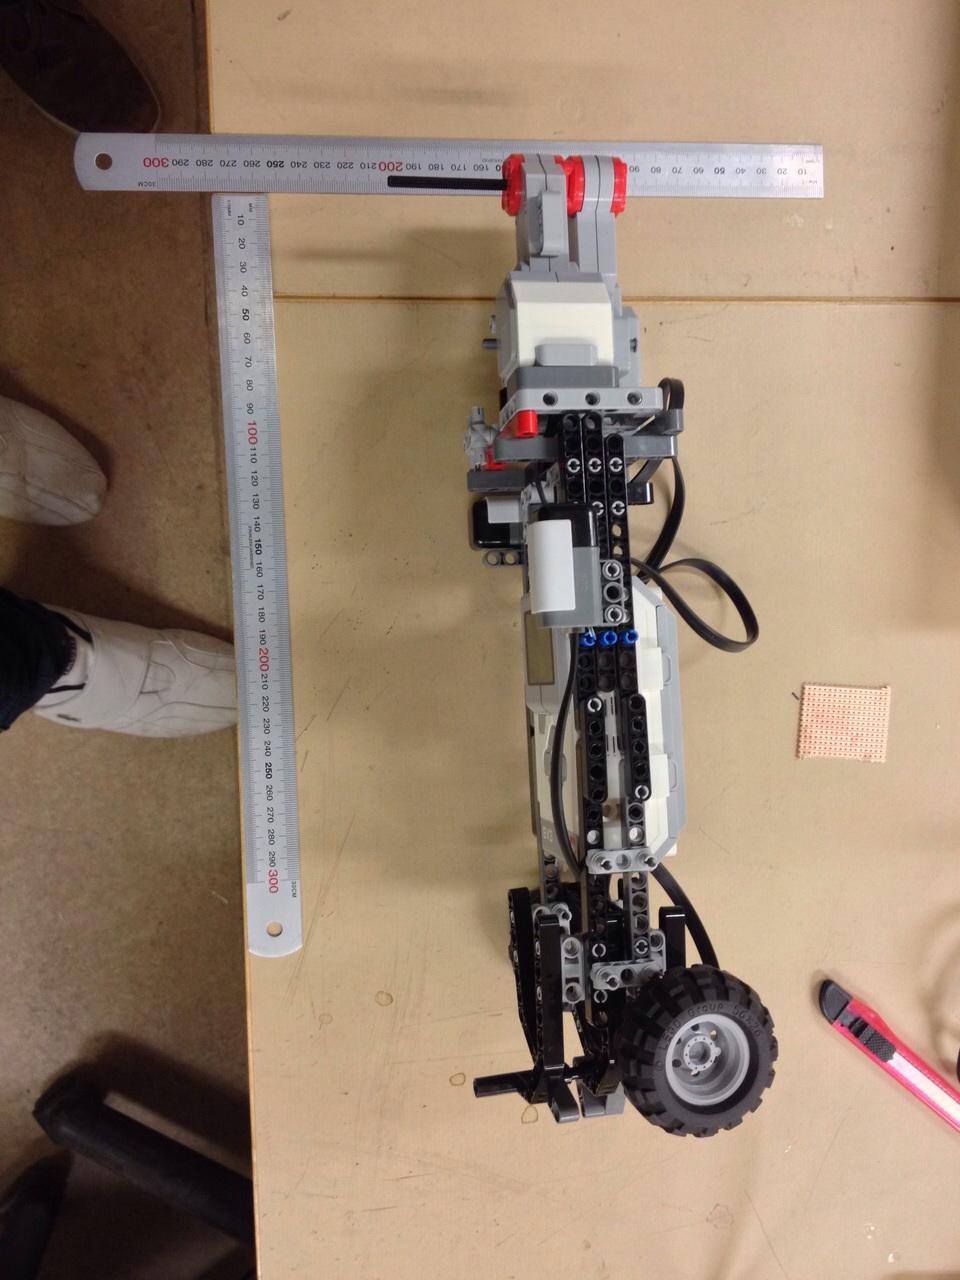
\includegraphics[width=0.35\textwidth,height=0.25\textheight]{prototype_2_a}} 
	\subfloat[]{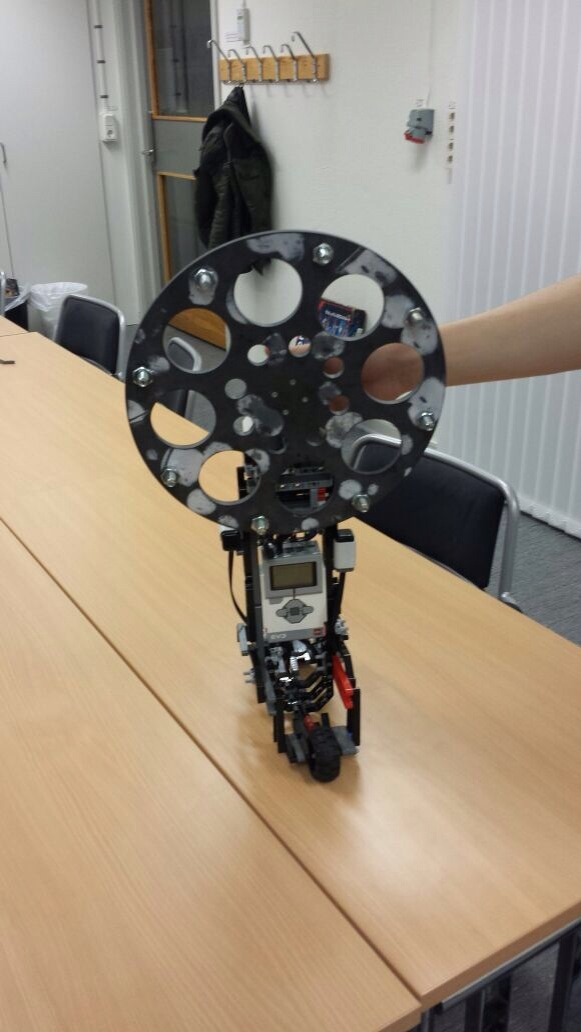
\includegraphics[width=0.35\textwidth,height=0.25\textheight]{prototype_2_b}} 
	\subfloat[]{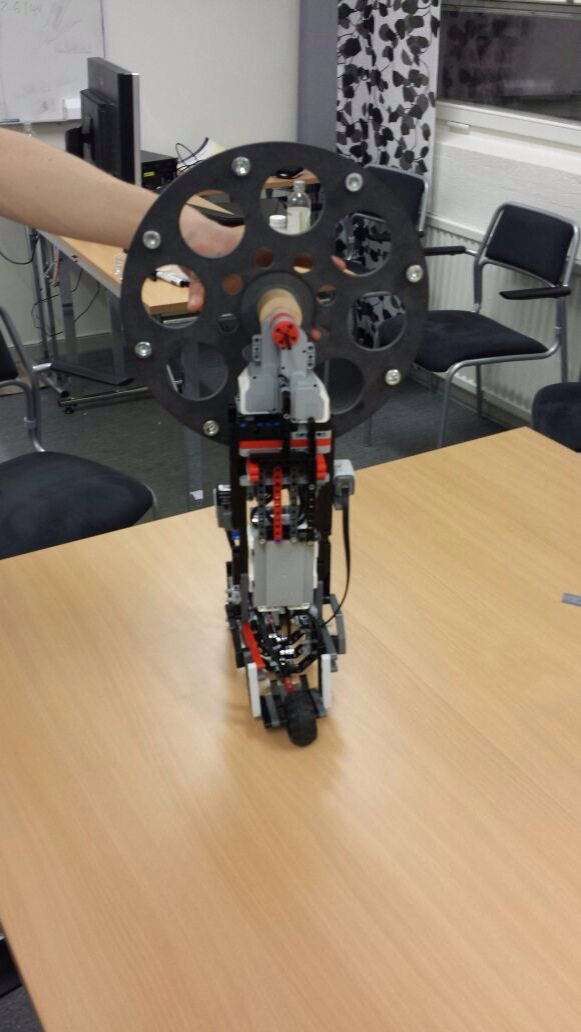
\includegraphics[width=0.35\textwidth,height=0.25\textheight]{prototype_2_c}}  
	\caption{Shows the second prototype from different angles with the first prototype of the reaction wheel.}
    \end{figure}
    
        \begin{figure}[h]
        \center
	 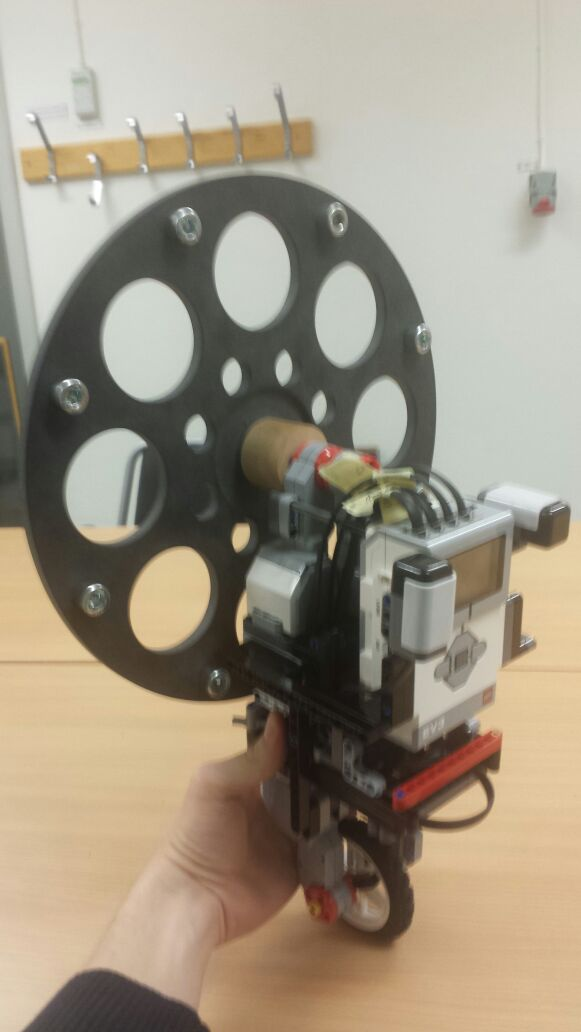
\includegraphics[width=0.5\textwidth,height=0.5\textheight]{prototype_3_a}
	\caption{Shows the third prototype with the first prototype of the reaction wheel.}
    \end{figure}
    
      \begin{figure}[h]
      	\center
	\subfloat[]{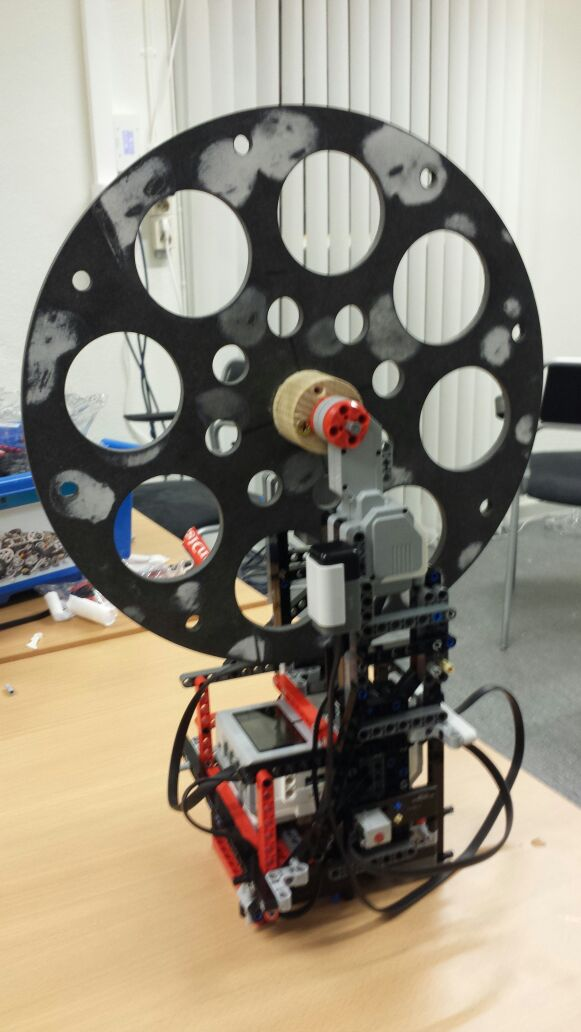
\includegraphics[width=0.35\textwidth,height=0.30\textheight]{prototype_4_a}} 
	\subfloat[]{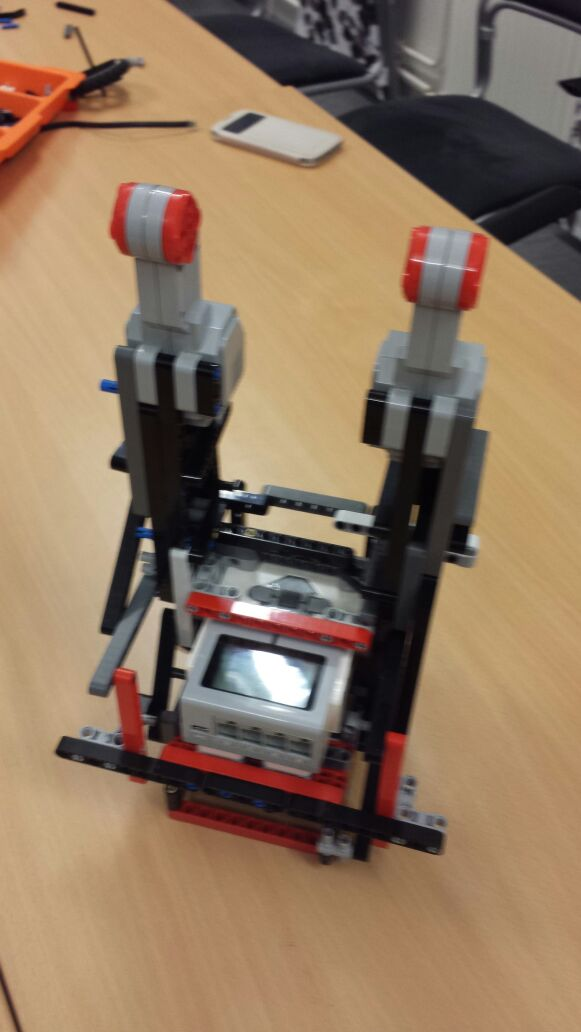
\includegraphics[width=0.35\textwidth,height=0.30\textheight]{prototype_4_b}} 
	\caption{Shows the fourth prototype from different angles with the first prototype of the reaction wheel.}
    \end{figure}
    
    
    
    \subsubsection{More details about the prototypes}
    
    We spent a lot of time to build several different prototypes for multiple reasons and solutions. in the beginning of the project we demonstrated some rough prototype. With regards to some requirements and limitations therefore most of the constructions we tried did not admire our lego unicycle. \\
    
    Lets look the first prototype of the project. in the very beginning of the project we designed the prototype which is attached bellow. This was built before we got the reaction wheel. with this prototype the reaction wheel was decided to be connected to the top and front part of the EV3 as seen in the Figure \ref{fig:prototype_1}. 
    
    
  \begin{figure}[h]
   \center
	\subfloat[]{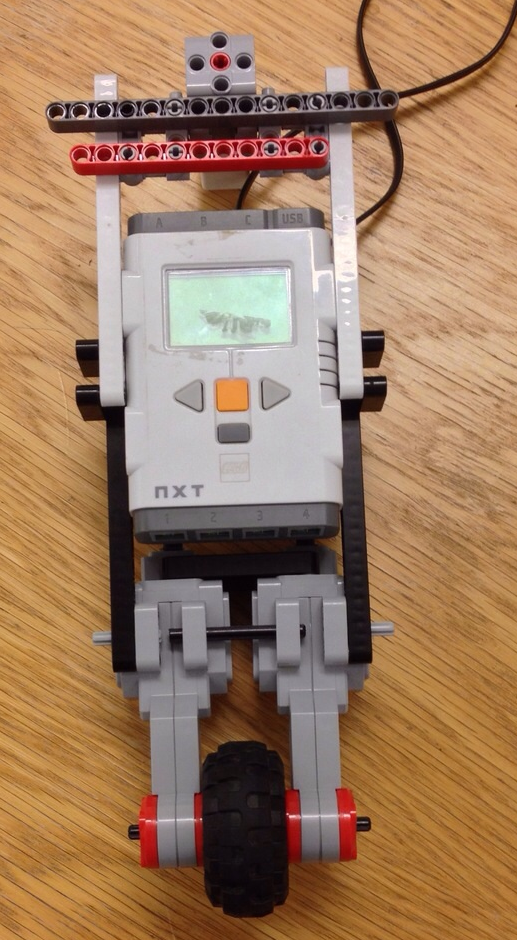
\includegraphics[width=0.3\textwidth,height=0.3\textheight]{Prototype_1_a.png}} 
	\subfloat[]{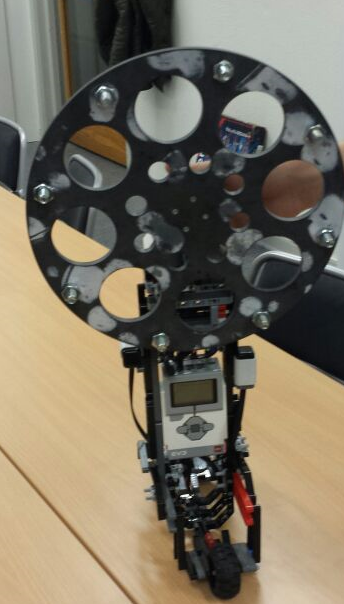
\includegraphics[width=0.3\textwidth,height=0.3\textheight]{Prototype_1_b.png}}  
	\caption{Shows the first prototype with and with out the reaction wheel.}
    \label{fig:prototype_1}
  \end{figure}
  
  We got some  problems due to weight balancing and torque tolerance of the reaction wheel for this design since the reaction wheel weighed more then the lego unicycle, the problem showed up when connected the reaction wheel. the reaction wheel made the unicycle want to fall front and thereafter the reaction wheel torn out  due to the stress caused by the max torque. this was a big problem which we couldn't solve with this prototype. therefore we changed this prototype and started building a new one.
 According to the previous construction we have some requirements and specifications that our new prototype should be able to fulfill since we couldn't solve all those problems with the previous prototype.

This construction we focused on building a prototype which folds the reaction wheel backwards to enable the reaction wheel tolerate the stress and not torn out.since the EV3 weighs more as well, we have decided to build the prototype as shown in figure \ref{fig:prototype_2}. to compensate the weight of the reaction wheel connecting to the top and front of the unicycle.

\begin{figure}[h]
        \center
	 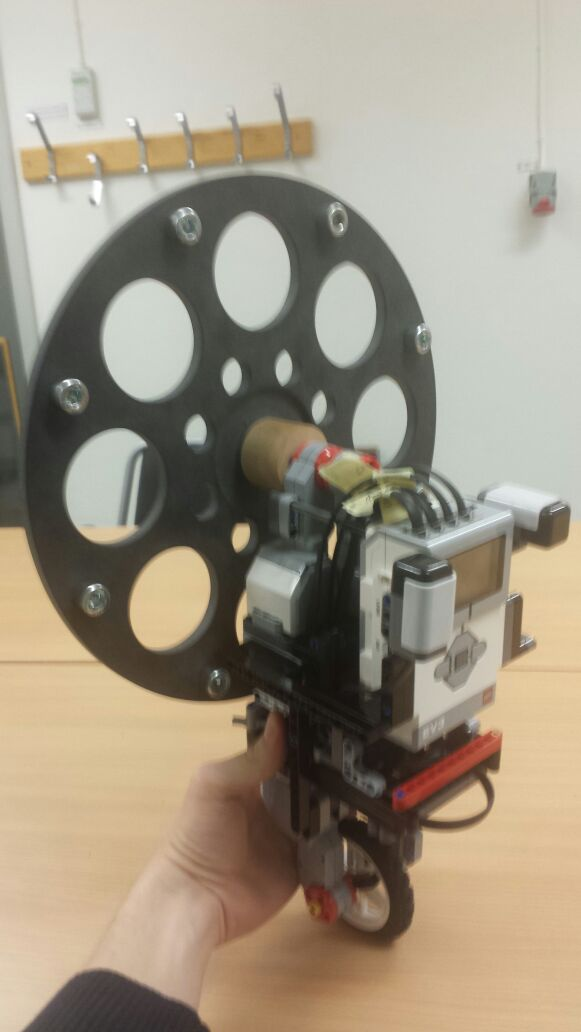
\includegraphics[width=0.3\textwidth,height=0.3\textheight]{IMG-20141215-WA0000__1_.jpg}
	\caption{Prototype 2}
    \label{fig:prototype_2}
    \end{figure}

The result of the lately construction didn't give much better solution. the construction couldn't handle the stress due to the reaction wheel, furthermore the motor which is connected to the reaction wheel torn out, the weight balancing problem was not solved as expected either. therefore we once more decided to build another prototype which will achieve our requirements.

Since the last two construction failed on our requirements therefore we have tried another approach to solve those issues. this time we got to rebuild both the reaction wheel and the prototype. we designed reaction wheel with two motors connecting from both sides as seen in figure \ref{fig:prototype_3}.
To connect this time the reaction wheel above the EV3 and between two motors connecting from both sides and holding to prevent the reaction wheel to dismantle. 

 \begin{figure}[h]
   \center
	\subfloat[]{\includegraphics[width=0.3\textwidth,height=0.3\textheight]{Prototype_3_a.jpg}} 
	\subfloat[]{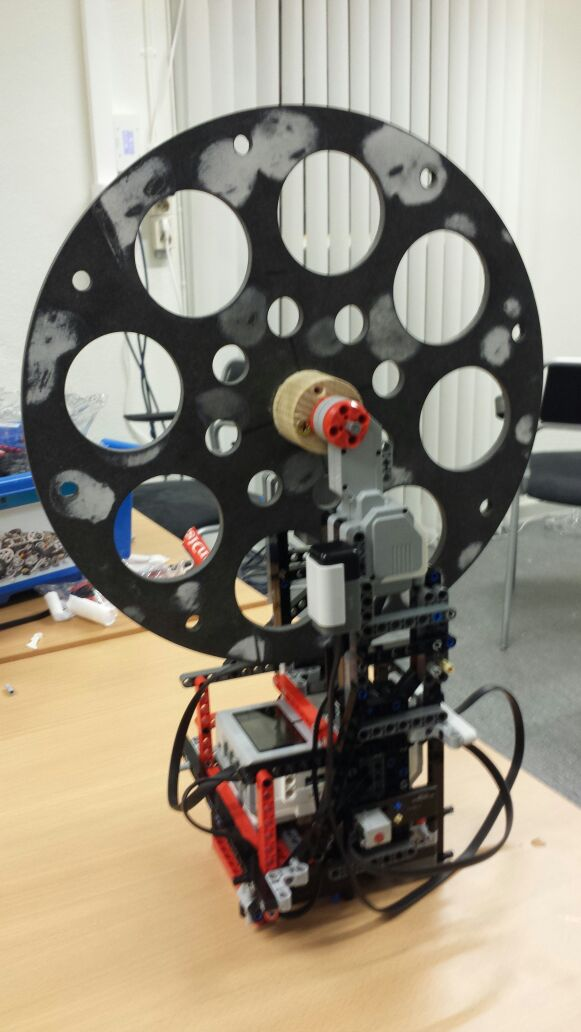
\includegraphics[width=0.3\textwidth,height=0.3\textheight]{Prototype_3_b.jpg}}  
	\caption{Shows the third prototype with and with out the reaction wheel.}
	\label{fig:prototype_3}
  \end{figure}
  
  This final construction coped with all the requirements that is to say this design handled the stress accurately and prevented the reaction wheel to dismantle.
    
    
    
    
    
\newpage
\section{Modeling}
\label{sec:Modeling}
	\subsection{Lateral Balance}
	
	We realized early in the project that controlling the inertia wheel is the most complicated part of the project. The complexity comes from several areas. The sensors have to be very accurate (which they are not), the simulation in simulink had to take account of the relationship between torque and the speed of the wheel among other things, we had to design a working controller.

The unicycle is similar to an inverted pendulum with a point mass in the center of mass, with an additional mass that is the inertia wheel, seen in figure 17. We modeled the pendulum as can be seen in (1). The relevant states from the model are the angle of the pendulum, the the angular velocity of the pendulum and the angular velocity of the inertia wheel. The angular position of the inertia wheel is not important as only the change in angular position affects the torque. Torque is the momentum you get when a vector force is acted on the wheel with a certain radius. The torque acting on the pendulum due to gravity (which makes it fall) must be less that the torque from the inertia wheel (which we can control) for it to be stable. The reaction torque is therefore dependent on the radius of the wheel. The maximum torque of the engine is also limited, so some angles are impossible for the reaction wheel to stabilize.


\begin{figure} [h]
	\centering
	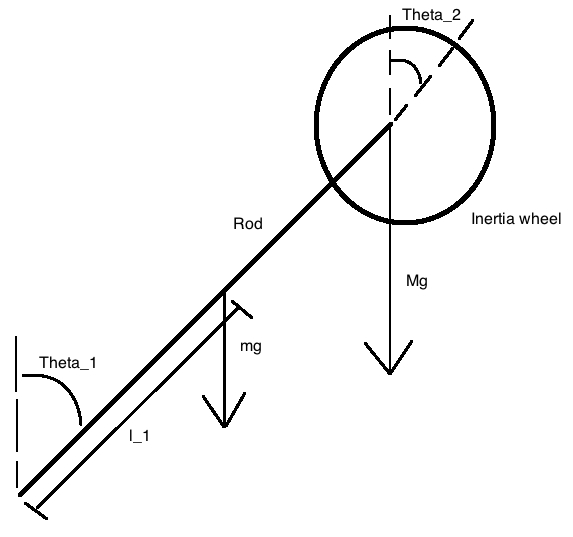
\includegraphics[width=0.7\textwidth]{Inverted_pedulum_2}
	\caption{Shows the sketch of the inverted pendulum}
	\label{fig:sketch_inverted_pendulum}
\end{figure}

\newpage	
	
		\subsubsection*{Mathematical model}
		
The principle idea of this control problem is to receive a reaction torque from the inertia wheel that is larger than the torque exerted on the unicycle from gravity. Looking at figure 17 we see the forces acting on the unicycle as it 	falls. If we assume that all the mass of the body exists in one point, the center of mass, the model of the process can be calculated using Newtons laws. The use of Newtons laws was chosen instead of the Lagrangian equations because it would give an adequately accurate model while still being easier to determine. 

The angular acceleration of the body will equal the net torque acted on the center of mass and the center of the inertia wheel due to gravity, and the reaction torque opposing the other two. The reaction torque is caused by the angular acceleration of the inertia wheel. Controlling the reaction torque in such a way that will keep 	          $ \frac{\partial^2 \theta_{b} }{\partial t^2}  = 0 $ and $\theta_{b}=0$ will make the system stable. It was estimated that the friction from the EV3 motor would we small and it was neglected from the equations.

		
		\begin{equation}
		\begin{aligned}
	     	 (J_{w}+ML^2 + J_{b} ) \frac{\partial^2 \theta_{b} }{\partial t^2}  &= l_{1} \sin{\theta_{b}} m g + L \sin{\theta_{b}} M g - \tau    \\  
		 J_{w} \frac{\partial^2 \theta_{w}} {\partial t^2} &= \tau
		\end{aligned}
	 	\label{equ:inverted_pendulum}  
\end{equation}
				
Where $\theta_{b}$ is the angle of the body, $\theta_{w}$ is the angle of the inertia wheel, $J_(b)$ and $J_(w)$ is the moment of inertia of the body and the wheel, $m$ is the mass of the body without the wheel, $M$ is the mass of the wheel, $g$ is the gravitational constant, $l_{1}$ is the length from the pivot point to the center of mass, $L$ is the length of the pivot point to the center of the wheel and $\tau$ is the reaction torque.

As stated before the interesting states are the angle of the body, the angular speed of the body and the angular speed of the wheel. The model in (1) can be linearized around the origin where $\theta_{b}=0$. When the angle of the body is close to zero $sin(\theta_{b})\approx\theta_{b}$. Since the angle of the body will mainly be close to zero with the right controller the approximation will serve for the model. The new model and state space representation linearized around the origin will be:

		\begin{equation}
		\begin{aligned}
	     	 (J_{w}+ML^2 + J_{b} ) \frac{\partial^2 \theta_{b} }{\partial t^2}  &= l_{1} \theta_{b} m g + L \theta_{b} M g - \tau    \\  
		 J_{w} \frac{\partial^2 \theta_{w}} {\partial t^2} &= \tau
		\end{aligned}
	 	\label{equ:inverted_pendulum}  
\end{equation}

$x_{1}$: Angle of the body \\
$x_{2}$: Angular velocity of the body\\
$x_{2}$: Angular velocity of the inertia wheel\\

		\begin{equation}
		\begin{aligned}
		\dot{x_{1}} = x_{2}\\
		\dot{x_{2}} = \frac{g }{(J_{w}+ML^2 + J_{b} )}(l_{1}m + LM)x_{1} - \frac {1}{(J_{w}+ML^2 + J_{b} )} \tau \\
		\dot{x_{1}} = \frac {1}{J_{w}} \tau\\
		\end{aligned}
	 	\label{equ:inverted_pendulum}  
\end{equation}




$A =  \begin{bmatrix} 
0 & 1 & 0 \\
\frac{g }{(J_{w}+ML^2 + J_{b} )}(l_{1}m + LM) & 0& 0 \\
0 & 0 & 0 
 \end{bmatrix}$
 
 $B =  \begin{bmatrix} 
0 \\
-\frac {1}{J_{w}} \\
\frac {1}{J_{w}}
 \end{bmatrix}$
 
  $C =  \begin{bmatrix} 
1 & 0 & 0\\
0 & 1 & 0\\
0 & 0 & 1\\
 \end{bmatrix}$
 
 $D=0$
 
 
 
 \subsubsection*{Controller and Simulink}
 
 \begin{figure} [h]
	\centering
	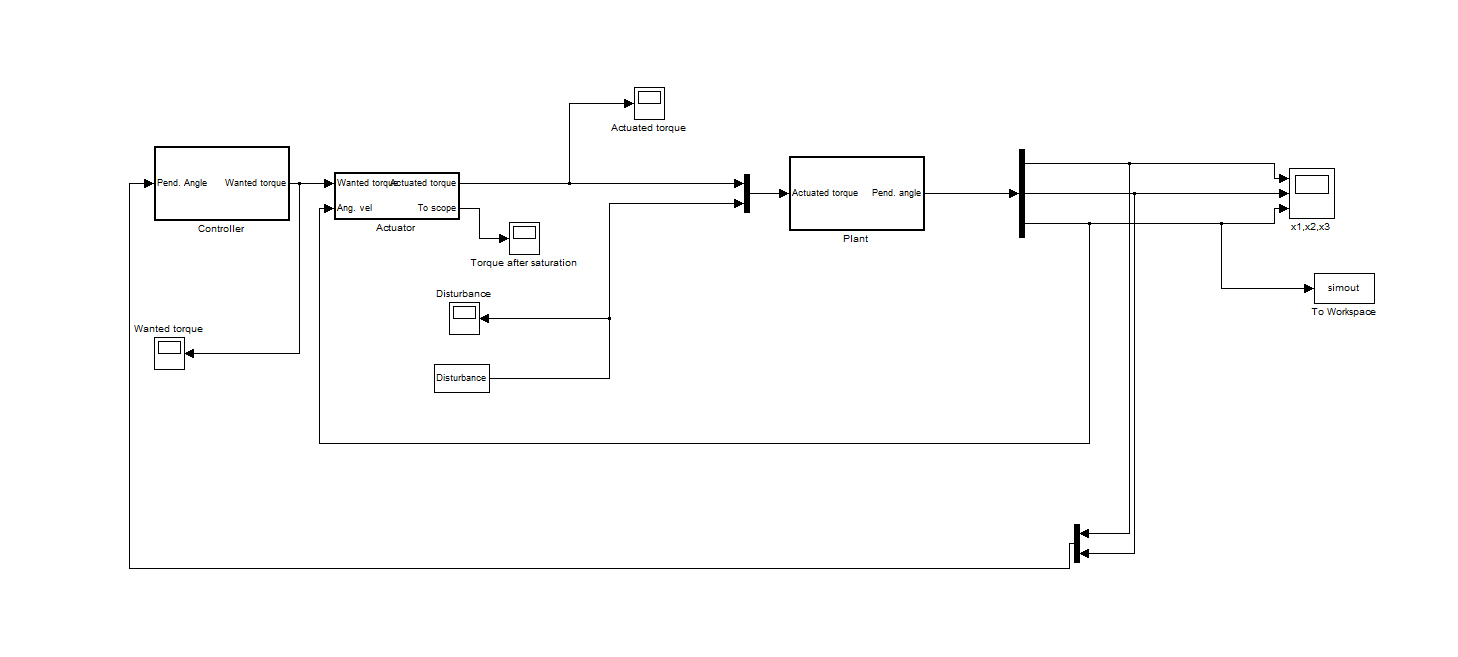
\includegraphics[width=0.7\textwidth]{SimulinkInertia.png}
	\caption{The simulink model}
	\label{fig:sketch_inverted_pendulum}
\end{figure}
 
 When creating the simulink model we had to take some physical limitations into account. First, the torque exerted by the motor will not always equal its reference value. The reason being that the torque will decrease as the angular speed of the wheel increases according to the formula:
 
 
 		\begin{equation}
		\begin{aligned}
\tau_{real} = \tau_{ref}(1-k\dot{\theta_{w}})
		\end{aligned}
	 	\label{equ:inverted_pendulum}  
\end{equation}
 
The maximum torque that can be exerted by the motor is also limited. It was determined that $\tau_{max}=0.384$. Using two motors the max torque is therefore $\tau_{max2}=0.768$. There was also a disturbance that had to be taken into account. The disturbance can be seen as a separate input to the process, as an acceleration exerted on the body.

  $B_{dist} =  \begin{bmatrix} 
0\\
1\\
0\\
 \end{bmatrix}$
  
 Two controllers were tested for the model. A PID controller and an optimal controller determined through the LQG method. The advantage with the PID controller was that its parameters could be tuned using a block in simulink called "PID Tuner". A stable closed loop system was achieved with the controller:
 
 

 		\begin{equation}
		\begin{aligned}
C= P + \frac{I}{s} + D\frac{N}{1+N\frac{1}{s}}
		\end{aligned}
	 	\label{equ:inverted_pendulum}  
\end{equation}

\newpage

$P=73$\\
$I=65$\\
$D=7.5$\\
$N=238$\\

The controller is, however, not stable. The angular velocity of the inertia wheel will continue to increase until it reaches it's maximum value, then the unicycle will fall.
An optimal controller was needed to stabilize the system. To optimize the controller we implemented a linear quadratic regulator which minimizes the cost function, seen in (6). The Q matrix determines how much each state will be penalized. Since we want to keep cost function (J) small a large Q will require that the states are small. Q=[q1 0 0; 0 q2 0; 0 0 q3]. The cost function we needed to minimize was:

\begin{equation}
		\begin{aligned}
	     	 E(x^TQx + u^TRu)
		\end{aligned}
	 	\label{equ:inverted_pendulum}  
\end{equation}

We set the weight matrices to the values:

\begin{itemize}

\item[] q1 = 1/1.57
\item[] q2 = 1/0.349
\item[] q3 = 1/16
\item[] R = 1/0.348

\end{itemize}

Which gives:

$L= [-32.4 -5.1 -0.22]$


These values come from the bounds of the states. The pendulum angle has a range of -1.57 to 1.57 radians (-90 to 90 degrees). We estimated that the maximum speed of the pendulum from free fall is 0.349 rad/s (about 20 degrees per second). The maximum angular velocity of the reaction wheel was determined to be 16 rad/s. Max torque is 0.348 Nm.
These values are used to normalize each product of the cost function so they are approximately equal. These values can be tuned to better performance with the real process.
With this controller the system became stable up to initial values of 2 degrees, or a disturbance of 1 Nm.

\begin{figure} [h]
	\centering
	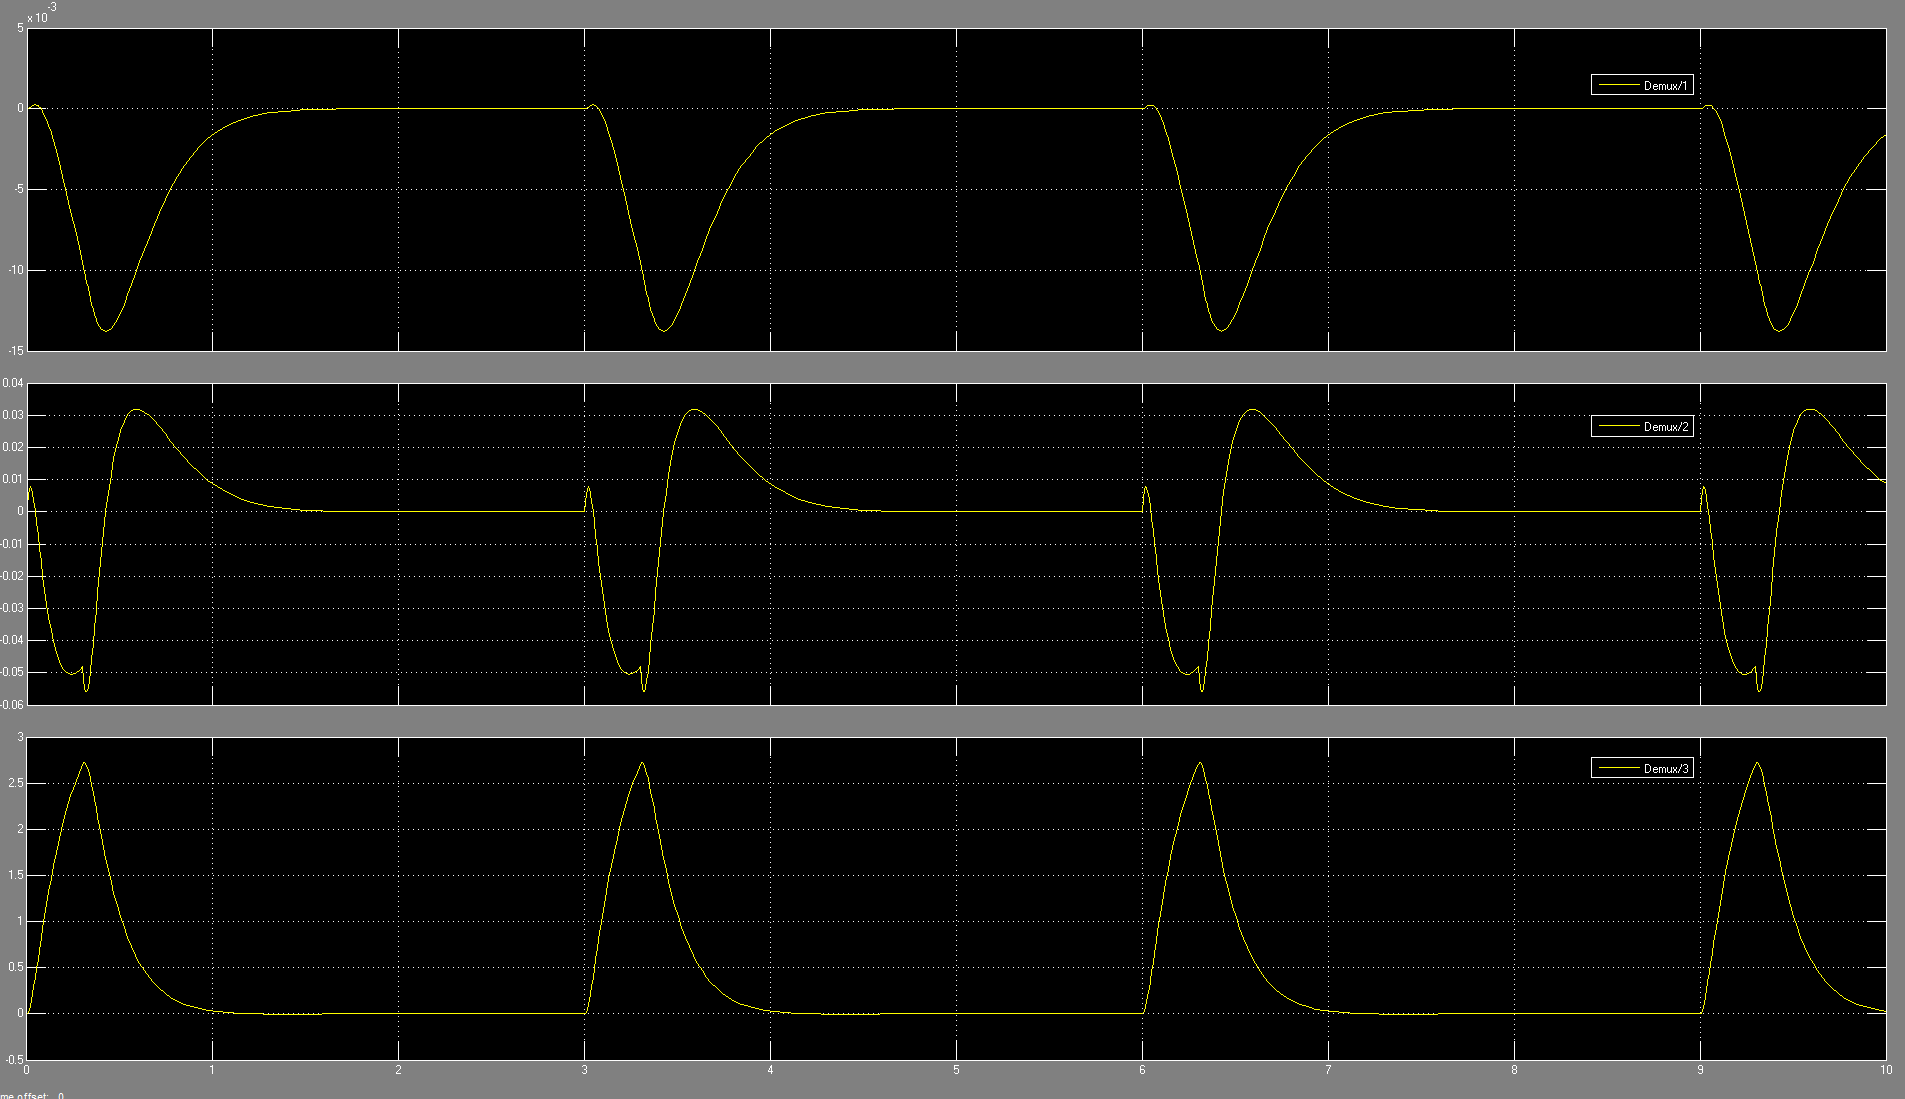
\includegraphics[width=0.7\textwidth]{plottttttt.png}
	\caption{The system when the disturbance is 1 Nm}
	\label{fig:sketch_inverted_pendulum}
\end{figure}


        
\section{Implementation}
	\subsection{Programs}
	% PROGRAMS SECTION
	In this section we will consider looking at the different programs and why the specific formats and programs where chosen as can bee seen in table \ref{table:Programs_used}. The OS (operating system) windows 7 was chosen due to the easiest setup guides on the internet for Lejos (the main programing language ). Lejos for main programing language was mainly used due to the familiarity of java, Lejos is a extension of java. It also has a class for every unit which was used in the project in other words made it easy to work with. Lejos had also support for parallel threads which other programs had difficulties with. Eclipse was the right deal for us because of the familiarity of it's functions and appearance. As well as the easy to use with EV3 because of one function that compiled, downloaded and ran the java program in in the EV3 with one button in the GUI. \\ The communication was made possible thru WinSCP and the only program that we could get working with EV3 and the desktop computer. The function that allowed us to drag and drop files from and to the EV3 was one of the major advantages with the given program. The format for transmitting data from measurements was "txt" because of the class DataLogger which handled it, txt is also easy to use in matlab so therefore it was the one to use. The DataLogger was the class which made it possible to transmit data in a easy fashion but also was not to complicated to upgrade which we also did. The original DataLogger class can been found in appendix \ref{Appendix:DataLogger_Orginal} while the modified can be found at Appendix \ref{Appendix:DataLogger_Modified}. Bluetooth was chosen because that was the only one that worked at the time and was the easiest to use because of the amount of aid on the internet regarding connection thru bluetooth.
	
	
	
	
	\begin{table}[h]
		\begin{tabular}{|c|c|c|}
			\hline
			OS & Programing language & GUI \\ \hline 
			Windows 7 & Lejos \cite{Lejos} & Eclipse \cite{Eclipse} \\ \hline  \hline \hline
			Communication GUI & Communication format & Communication medium \\ \hline
			Winscp \cite{WinScp} & txt -format & Bluetooth \\ \hline \hline \hline 
			Data- caption & - & - \\\hline
			DataLogger \cite{DataLogger}  & - & - \\ \hline	
		\end{tabular}
		\caption{Shows the programs and important formats which was used in the project.}
		\label{table:Programs_used}
	\end{table}
    
\section{Results}
\label{sec:results}
%RESULTS

The results of the project can bee seen in figures \ref{fig:plot_comp_filter_control_signal_19_Dec}, \ref{fig:plot_comp_filter_control_signal_3_Jan}, \ref{fig:plot_parallel_threads_two_sensors} and \ref{fig:plot_parallel_threads_IMU}. The figure \ref{fig:plot_comp_filter_control_signal_19_Dec} shows the first control signal that were sampled and the figure \ref{fig:plot_comp_filter_control_signal_3_Jan} shows the last one to be sampled with improvments. However the figures \ref{fig:plot_parallel_threads_two_sensors} and \ref{ig:plot_parallel_threads_IMU} was the results with the improvements by using paralled threads. As can be seen there where was no improvement in the u

  \begin{figure}[h]
		%\centering
		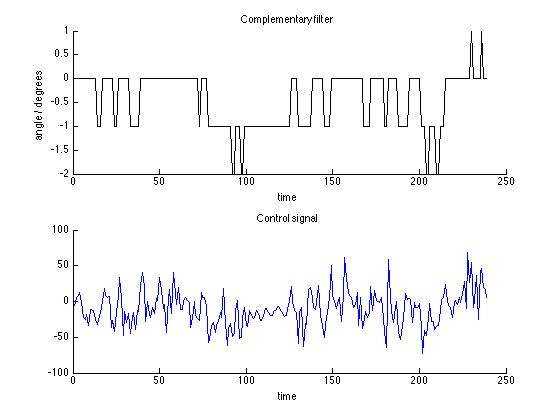
\includegraphics[width=1.3\textwidth]{comp_filter_control_signal_20150112_19_Dec}
		\caption{Shows the relation between the complementary filter and the control signal.}
		\label{fig:plot_comp_filter_control_signal_19_Dec}
  \end{figure}
  
  

   \begin{figure}[h]
		%\centering
		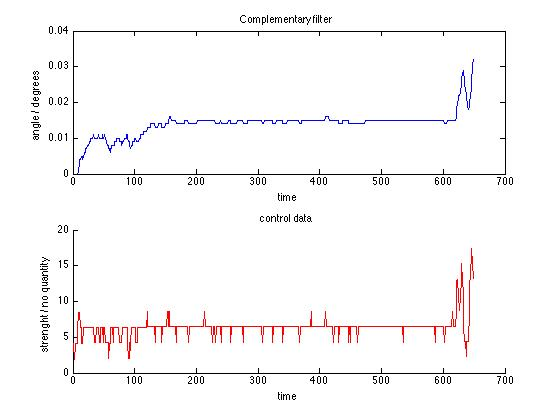
\includegraphics[width=1.3\textwidth]{comp_filter_control_signal_20150112_3_Jan}
		\caption{Shows the time taken for the two sensors to update their values with parallel threads.}
		\label{fig:plot_comp_filter_control_signal_3_Jan}
  \end{figure}
  
     \begin{figure}[h]
		%\centering
		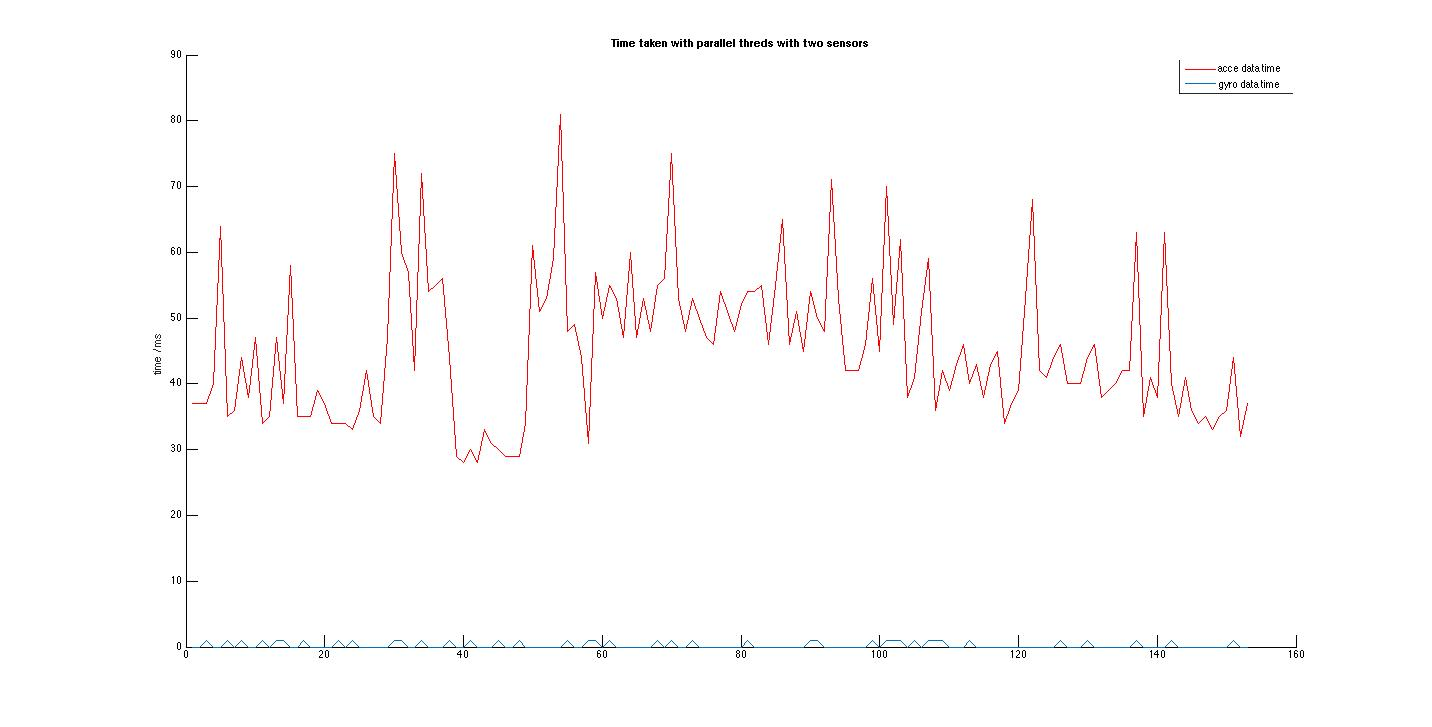
\includegraphics[width=1.4\textwidth]{parallel_threads_two_sensors_01}
		\caption{Shows the time taken for the IMU sensor to update its values with parallel threads.}
		\label{fig:plot_parallel_threads_two_sensors}
  \end{figure}
  
  
   \begin{figure}[h]
		%\centering
		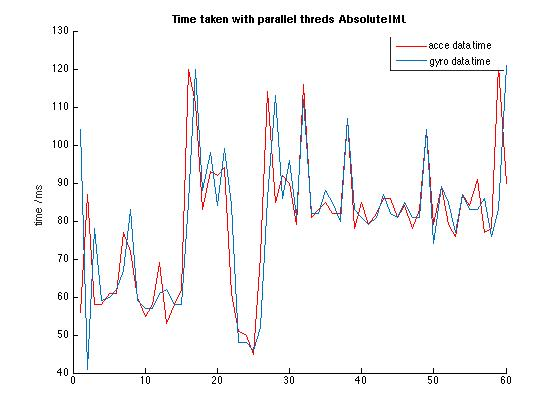
\includegraphics[width=1.4\textwidth]{parallel_threads_IMU}
		\caption{Shows the relation between the complementary filter and the control signal.}
		\label{fig:plot_parallel_threads_IMU}
  \end{figure}
  
  
  
  
  
  
  
  
	





\clearpage
\section{Conclusion}
In this section we will briefly go through some conclusions we draw from this project. First one being the Lejos main program is to slow for this kind of processes because of the many programs being nested. Java is not recommended for this kind of processes in general. Another problem we encountered was that the microprocessor was to slow due to slow reactions times in the program that uses parallel threads. A remark is also that then we used the IMU sensor it was to slow which was not expected. Further we can also se in the plots under section\ref{sec:results} that the engines are not being as strong as they should be due to the saturation due the power control. Because the control signal should according to the simulation be bounded by -0.42 to 0.42 but in reality we see that the control signal goes outside that region almost immediately. Lastly we can bring up that we did not have time to do the medial balance control due to many limitations of the hardware and the software.


\clearpage
\appendix

\section{Lejos Source Code}
\label{Appendix:Lejos Source Code}
\subsection{The main source code}
\label{Appendix:The_main_source_code}
\begin{lstlisting}

import java.util.ArrayList;
import java.util.List;

import lejos.hardware.sensor.HiTechnicAccelerometer;
import lejos.hardware.sensor.HiTechnicGyro;
import lejos.hardware.sensor.MindsensorsAbsoluteIMU;
import lejos.hardware.port.MotorPort;
import lejos.hardware.port.SensorPort;
import lejos.hardware.lcd.LCD;
import lejos.hardware.motor.NXTMotor;
import lejos.hardware.Button;
import lejos.robotics.SampleProvider;

public class RealCodeInertia2015 {


		static final long h= 30;
	    // sleep can only take in long which is bounded, greater than zero
		//static final long h = 5;
		
		private static final float Ku = 0.0042f*((1/0.05f));
		
		static final float phi11 = 1.0192f;
		static final float phi12 = 0.0302f;
		static final float phi21 = 1.2844f;
		static final float phi22 = 1.0192f;
		static final float phi33 = 1f;
		
		static final float gamma1 = -0.0112f;
		static final float gamma2 = -0.7507f;
		static final float gamma3 = 7.8431f;

		static final float l1 = -13.7278f;
		static final float l2 = -2.1648f;
		static final float l3 = -0.0750f;
		
		      
		
		static final float a = 1.214454545454f;
	
		
		

		static float u = 0.0f;

		static int power = 0;

		static float x1,x2,x3;

		static float x1Old =0.0f;
		static float x2Old= 0.0f;
		static float x3Old = 0.0f;
	
		//For the acce meter
		static MindsensorsAbsoluteIMU sensor = new MindsensorsAbsoluteIMU(SensorPort.S1);
		static SampleProvider AcceMode;
		static SampleProvider RateMode;
		static List<Integer> acceTime = new ArrayList<Integer>();
		static List<Integer> gyroTime = new ArrayList<Integer>();
		static DataLogger dl;
		
		
		static float[] sample_Acce = new float[3]; 
		static double rad_Acce;
		static double radians;
		
		// For the gyroscope
		static  float angle_Gyro=0;
		static float angleOffset=0;
		//static HiTechnicGyro gyro =new HiTechnicGyro(SensorPort.S2 ); 
		static float angle_of_set;
		static float[] sample = new float[1];
		static float offset_gyro=0f;
		static float offset_acce=0f;
		static float sample_1=0f;
		
		// For the complementary filter
		static float comp_filter_angle=0;
		static float A = 0.95f;
		static float count;
		
		//Wheel Speed
		static float speed_W=0;
		
		static long time;
		static long tAfterLogWrite;
		static long[] data;
		
		static List<Integer> listGlobalTime = new ArrayList<Integer>();
		static List<Integer> listTimeAcce = new ArrayList<Integer>();
		static List<Integer> listTimeGyro = new ArrayList<Integer>();
		static List<Integer> listTimeComp = new ArrayList<Integer>();
		static List<Integer> listPrecStates = new ArrayList<Integer>();
		static List<Integer> list_gyro_angle = new ArrayList<Integer>();
		
		
		// The values of acce_sample, gyro_sample, control signal, compl_filter, offset
		static List<Integer> listAcce = new ArrayList<Integer>();
		static List<Integer> listGyro = new ArrayList<Integer>();
		static List<Integer> listControl = new ArrayList<Integer>();
		static List<Integer> listComp = new ArrayList<Integer>();
		static List<Integer> listWheel = new ArrayList<Integer>();
		
		// The values of the offset
		
		static List<Integer> listoffset = new ArrayList<Integer>();
		static List<Integer> listoffset_acce = new ArrayList<Integer>();
		
		
		
		
		
		public static void main(String[] args) throws InterruptedException{
			AcceMode= sensor.getAccelerationMode();
			RateMode= sensor.getRateMode();
			//INIT PROGRAM
	
			LCD.drawString("Initialize Calibrate", 0, 1);
			
			Button.waitForAnyPress();
			
			calc_offset_gyro();
			calc_offset_acce();
			LCD.clearDisplay();
			LCD.drawString("Press to start", 0, 1);
			Button.waitForAnyPress();
			LCD.clearDisplay();
			NXTMotor m1 = new NXTMotor(MotorPort.A);		
		        NXTMotor m2 = new NXTMotor(MotorPort.B);
		    
			count=0;
			
			//INIT PROGRAM 
			DataLogger dl = new DataLogger("sample.txt"); 
			
			//SampleProvider accelerationProvider= accelerationSensor.getAccelerationMode();
			long t = System.currentTimeMillis();
			long t_before;
		while(Button.ESCAPE.isUp()){
			
			time = System.currentTimeMillis();
		
	

			/////////////////////////////////////////////////
			////////compute angles///////////////////////////
			/////from the complementary filters/////////////
			///////////////////////////////////////////////
			
			
			 t_before = System.currentTimeMillis();
			 
				float[] sampleAcce = new float[AcceMode.sampleSize()];
				
				AcceMode.fetchSample(sampleAcce, 0);
			
			   

				
			  rad_Acce =  (sampleAcce[0]/9.81)- offset_acce ;
			  listAcce.add( (int) (sampleAcce[1] * 1000f)  ) ;  // TODO Needs to be converted back in the plot script
			  //double rad_Acce = Math.toRadians(angle_Acce);
			  //long timeAccel = System.currentTimeMillis() - t_before;
			  
			  
			  
			  // The gyro time
			 // t_before = System.currentTimeMillis();

				float[] sampleGyro= new float[RateMode.sampleSize()];	
				
				RateMode.fetchSample(sampleGyro,0);
		      sample_1 = sampleGyro[0]  - offset_gyro; 
		      double rad_gyro = Math.toRadians(sample_1);
		      
		      listGyro.add((int) ( sample_1*(1000f) ) );   	// TODO Needs to be converted back in the plot script
		      
		      
		      //long timeGyro =System.currentTimeMillis()-t_before ;
		      
			
		      
		      // The complementary filter
		      //t_before = System.currentTimeMillis();
			  comp_filter_angle = (float) (A * (comp_filter_angle + rad_gyro * 0.04) + (1-A)*(rad_Acce)) ;
			  listComp.add((int)  (   comp_filter_angle * (1000f)) ); // TODO Needs to be converted back in the plot script
	
			x1Old= comp_filter_angle; //==> from the complementary filters which is comp_filter_angle///// 
			
			x2Old = sample_1; //==> rate from the gyro - offset = sample_1 /////
			
			
			//LCD.drawString("Angle", 0, 0);
			//LCD.drawString("Ang vel", 1, 0);
			
			
		
			/////////////////////////////////////////////////////////
			///////Calculations of the wheel speed/////////////////
			/////////////////////////////////////////////////////
			
			 t_before = System.currentTimeMillis();
			 float radians_Wheel = (float) (m1.getTachoCount() *  ((Math.PI)/180));
			 //m1.resetTachoCount();
			 long time_wheel = System.currentTimeMillis()- t_before;
			  x3Old = (float) (radians_Wheel/(0.04)); // ==> speed of the wheel in radians /sec ==> x3Old
			listWheel.add((int)(x3Old));
			/////////////////////////////////////////////////
			//////////////compute control laws/////////////
			////////////////////////////////////////////////
			  
		     u = -1*( (l1 * x1Old) +( l2 * x2Old) +( l3 * x3Old) ) ;
		     listControl.add((int) ( u* (1000f)  ) ); // TODO Needs to be converted back in the plot script
		
			
			power = (int) ( (u) / Ku) ;
			if(power>100){
				power= 100;
			}

			if(power<-100){

				power= -100;
			}
			 // LCD.drawString(Integer.toString(m1.getTachoCount()), 0, 0);
				
			
			 t_before = System.currentTimeMillis();
			 m1.setPower(power);
			 m2.setPower(power);
			

			m2.backward();
			m1.backward();	
			long set_power_time =System.currentTimeMillis();
			
      
	
			//PreCalculate the next States
			
			x1 = phi11*x1Old+ phi12*x2Old + gamma1*(u);
			x2 = phi21*x1Old+ phi22*x2Old + gamma2*(u);
			x3 = phi33*x3Old+ gamma3*(u);
			
			x1Old=x1;
			x2Old=x2;
			x3Old=x3;
			long prec_states_time = System.currentTimeMillis()- set_power_time ;
			
			
            list_gyro_angle.add((int) (comp_filter_angle*(1000f)) );  // TODO Needs to be converted back in the plot script
			
		

			t=  t + h ;
			long duration= t - System.currentTimeMillis();
			
			if (duration > 0) {
				try {
					Thread.sleep(duration);
				} catch (InterruptedException e) {
					e.printStackTrace();
				}
			}
			
			
			
			
			long time2 = System.currentTimeMillis() - time ;
			
			
			listGlobalTime.add((int)time2);
			
			
			
			//listTimeGyro.add((int)timeGyro);
			
		//	listTimeComp.add((int)timeComp);
			
	//		listPrecStates.add((int)prec_states_time);
			
			
			
			//Button.waitForAnyPress();
			}
		
			m1.setPower(0);
			m2.setPower(0);
		
		   for(int a = 0; a < listGlobalTime.size()  ; a++){
			   
		    dl.writeSingleSample(listGlobalTime.get(a));
		    //dl.writeSingleSample(list_gyro_angle.get(a));
		     //dl.writeSingleSample(listTimeAcce.get(a));
		    //dl.writeSingleSample(listTimeGyro.get(a));
		    //dl.writeSingleSample(listTimeComp.get(a));
		    //dl.writeSingleSample(listPrecStates.get(a));
		    dl.writeSingleSample(listAcce.get(a));
		    dl.writeSingleSample(listGyro.get(a));
		    dl.writeSingleSample(listControl.get(a));
		    dl.writeSingleSample(listComp.get(a));
		     //dl.writeSingleSample(listWheel.get(a));
		     
		     if(listoffset.size() > a  ){
		    	 dl.writeSingleSample(listoffset.get(a));
		    	
		    	 
		     }else{
		    	 dl.writeSingleSample(0);
		    	
		     }
		     
		     if(listoffset_acce.size() > a  ){
		    	
		    	 dl.writeSingleSample(listoffset_acce.get(a));
		    	 
		     }else{
		    	 dl.writeSingleSample(0);
		    	 
		     }
		    
		    //dl.newLine();
		    
		   //}
		   
		   // write the offset in the end
		   dl.newLine();
		   }
		   dl.newLine();
		   dl.writeSingleSample((int) (offset_gyro*(1000f))  );		// TODO Needs to be converted back in the plot script
		   dl.newLine();
		   dl.writeSingleSample((int) (offset_acce*(1000f))  );
		   //END
		    m1.stop();
		    m2.stop();
		    m1.close();
		    m2.close();
			LCD.clear();
		    LCD.drawString("Program stopped", 0, 0);
		 
		}
	
		
		
		public static void calc_offset_gyro(){
			
			//LCD.drawString("Calibrate gyro", 0, 0);
			float temp_offset =0;
			int count = 100;
			for(int i =0;i<count ; i++){
				float[] sampleGyro= new float[RateMode.sampleSize()];	
				
				RateMode.fetchSample(sampleGyro,0);
				  listoffset.add((int) (sampleGyro[0] *(1000f) ) ); // TODO Needs to be converted back in the plot script
				  temp_offset = temp_offset + sampleGyro[0];
				  try {
					Thread.sleep(5);
				} catch (InterruptedException e) {
					e.printStackTrace();
				}
				  }
			
			offset_gyro= temp_offset/count;
			
		}
		
public static void calc_offset_acce(){
			
			
			//float[] sample_acce =  new float[3]; 

			float temp_offset = 0;
			int count = 100;
			for(int i =0;i<count ; i++){
				float[] sampleAcce = new float[AcceMode.sampleSize()];
				
				AcceMode.fetchSample(sampleAcce, 0);
				  temp_offset = temp_offset + sampleAcce[0];
				  int sample_acce_temp_write=(int) (sampleAcce[1] * 1000f);
				  listoffset_acce.add( (sample_acce_temp_write) ); // TODO Needs to be converted back in the plot script
				  LCD.drawString(Float.toString(temp_offset), 0, 0);
				  try {
					Thread.sleep(5);
				} catch (InterruptedException e) {
					e.printStackTrace();
				}
				  }
			offset_acce = temp_offset/count;
			
		}
	}

	
\end{lstlisting}
\subsection{DataLogger}
	\subsubsection{DataLogger Orginal}
	\label{Appendix:DataLogger_Orginal}
	\begin{lstlisting}
import lejos.hardware.lcd.LCD;
import lejos.ev3.*;

import java.io.*;
/**
 * A simple data logger that can be used to sample a sequence
 * of integer data values in a flash file. The
 * file is a text consosting of a sequence of lines with
 * a time value and a sample data value separated by a comma.
 * 
 * When data has been sampled the flash file can be transfered to a
 * PC by means of the tool nxjbrowse.
 * 
 * @author  Ole Caprani
 * @version 4.02.13
 */
public class DataLogger {
    private File f;
    private FileOutputStream fos;
    private int startTime;

    public DataLogger (String fileName)
    {
        try
        {	        
            f = new File(fileName);
            if( ! f.exists() )
            {
                f.createNewFile();
            }
            else
            {
                f.delete();
                f.createNewFile();
            }
             
            fos = new  FileOutputStream(f);
        }
        catch(IOException e)
        {
            LCD.drawString(e.getMessage(),0,0);
            System.exit(0);
        }
        startTime = (int)System.currentTimeMillis();
    }
    
    public void start()
    {
    	startTime = (int)System.currentTimeMillis();
    }
	
    public void writeSample( int time, float sample )
    {
		
        try
        {
            Integer timeInt = new Integer(time);
            String timeString = timeInt.toString();
            
            Float sampleInt = new Float(sample);
            String sampleString = sampleInt.toString();
            
            for(int i=0; i<timeString.length(); i++)
            {
                fos.write((byte) timeString.charAt(i));
            }
            
            // Separate items with comma
            fos.write((byte)(','));
            
            for(int i=0; i<sampleString.length(); i++)
            {
                fos.write((byte) sampleString.charAt(i));
            }

            // New line
            fos.write((byte)('\r'));
            fos.write((byte)('\n'));				

        }
        catch(IOException e)
        {
            LCD.drawString(e.getMessage(),0,0);
            System.exit(0);
        }
    }
    
    public void writeSample( float sample )
    {
    	writeSample((int)System.currentTimeMillis() - startTime, sample);
    }
    
    public void close()
    {
        try
        {
            fos.close();
        }
        catch(IOException e)
        {
            LCD.drawString(e.getMessage(),0,0);
            System.exit(0);
        }		 
    }
}
	\end{lstlisting}
	\subsubsection{DataLogger Modified}
	\label{Appendix:DataLogger_Modified}
	\begin{lstlisting}
	import lejos.ev3.*;
import lejos.hardware.lcd.LCD;

import java.io.*;
/**
 * A simple data logger that can be used to sample a sequence
 * of integer data values in a flash file. The
 * file is a text consosting of a sequence of lines with
 * a time value and a sample data value separated by a comma.
 * 
 * When data has been sampled the flash file can be transfered to a
 * PC by means of the tool nxjbrowse.
 * 
 * @author  Ole Caprani
 * @version 4.02.13
 * Modified by Group B
 */
public class DataLogger 
{
    private File f;
    private FileOutputStream fos;
    private int startTime;

    public DataLogger (String fileName)
    {
        try
        {	        
            f = new File(fileName);
            if( ! f.exists() )
            {
                f.createNewFile();
            }
            else
            {
                f.delete();
                f.createNewFile();
            }
             
            fos = new  FileOutputStream(f);
        }
        catch(IOException e)
        {
        	 LCD.drawString(e.getMessage(),0,0);
           
            System.exit(0);
        }
        startTime = (int)System.currentTimeMillis();
    }
    
    
    /* Sets the variable startTime to the current time*/
    
    public void start()
    {
    	startTime = (int)System.currentTimeMillis();
    }
	/* Writes a sample to a txt file
	  */
    public void writeSample( int time, int sample )
    {
		
        try
        {
        	// Make a string from the time 
            Integer timeInt = new Integer(time);
            String timeString = timeInt.toString();
            
            // Make a string from the sample
            Integer sampleInt = new Integer(sample);
            String sampleString = sampleInt.toString();
            
            /* Writes the time in the txt file (fos) */
            for(int i=0; i<timeString.length(); i++)
            {
                fos.write((byte) timeString.charAt(i));
            }
            
            // Separate items with comma
            fos.write((byte)(','));
            
            /* Writes the sample to the txt file */
            for(int i=0; i<sampleString.length(); i++)
            {
                fos.write((byte) sampleString.charAt(i));
            }

            // New line, makes no sense why have the both
            fos.write((byte)('\r'));
            fos.write((byte)('\n'));				

        }
        catch(IOException e)
        {
        	  LCD.drawString(e.getMessage(),0,0);
            System.exit(0);
        }
    }
    
    public void writeSample( int sample )
    {
    	writeSample((int)System.currentTimeMillis() - startTime, sample);
    }
    
    public void close()
    {
        try
        {
            fos.close();
        }
        catch(IOException e)
        {
            LCD.drawString(e.getMessage(),0,0);
            System.exit(0);
        }		 
    }
    
    /* Prepares a new line for more data to be written */
    public void newLine(){
    	// New line, makes no sense why have the both
    	try
    	{
    		fos.write((byte)('\r'));
            fos.write((byte)('\n'));
    	}
    	catch(IOException e)
    	{
    		 LCD.drawString(e.getMessage(),0,0);
           
    	}
    }
    
    /* Writes the single sample to the txt file and creates a comma at the end */
    public void writeSingleSample(int sample){
    	// Make a string form the sample
    	Integer sampleInt = new Integer(sample);
        String sampleString = sampleInt.toString();
    	
    	try
    	{
    		for(int i=0; i<sampleString.length(); i++)
            {
                fos.write((byte) sampleString.charAt(i));
            }	
    		 // Separate items with comma
            fos.write((byte)(','));
    	}
    	catch(IOException e)
    	{
    		 LCD.drawString(e.getMessage(),0,0);
    	}
    }
}
	\end{lstlisting}
	
	

\subsection{The sensor source test codes}
	\subsubsection{The gyroscope source test code}
	\label{Appendix:The_gyroscope_test_source_code}
	\begin{lstlisting}
	import lejos.hardware.Button;
import lejos.hardware.ev3.LocalEV3;
import lejos.hardware.lcd.LCD;
import lejos.hardware.port.Port;
import lejos.hardware.port.SensorPort;
//import lejos.hardware.port.SensorPort;
import lejos.hardware.sensor.EV3GyroSensor;
import lejos.hardware.sensor.HiTechnicAccelerometer;
import lejos.hardware.sensor.HiTechnicGyro;



public class Gyroscope {
	
	// Global variables
	   // HiTechnic sampel period is approx. 300 sampel/1 sek
	  static  float angle_Gyro=0;
	  static float angleOffset=0;
	  static HiTechnicGyro gyro;
	  static float angle_of_set;
	  static DataLogger dl = new DataLogger("Data_Gyro.txt");
	  static float[] sample = new float[1];
	  
	  
	public static void main(String[] args) throws InterruptedException {
		
	
		   LCD.drawString("Gyroscope_Program_Test", 0, 0);
		
		   Button.waitForAnyPress();
	        gyro = new HiTechnicGyro(SensorPort.S2 );
	       
	  
	     
	
	       get_Data_Gyro();
	       dl.close();
	       LCD.clear();
	       LCD.drawString("Program stopped", 0, 0);
	       Thread.sleep(2000);
		
		
	}
	
	public static void get_Data_Gyro(){
		while (! Button.ESCAPE.isDown())
	       {		   
	           
	    	   gyro.fetchSample(sample, 0);
	    	   
	    	   //calibrate the sample, deal with the offset assuming it is constant
	    	   sample[0] = sample[0];
	    	  angle_Gyro += (sample[0] * 0.003333333 ) ;
	    	   LCD.drawString("TestGyro", 3, 1);
	    	   LCD.drawString("Angle:", 0, 3);
	    	   LCD.drawString(""+angle_Gyro, 10, 4);
	    	   
	    	   LCD.drawString("sample", 0, 5);
	    	   LCD.drawString(""+sample[0], 10, 6);
	           dl.writeSample(sample[0]);   
	       }	
	}
	/* public static float calibrate(){
		 
		 float[] sampleCal = new float[1];
		 
		 for(int i=1; i<100; i++){
		 
			 gyro.fetchSample(sampleCal, 0);
		     angleOffset=  (angleOffset + sampleCal[0]);
	 }
		 
		 angleOffset= angleOffset/100;
		 
		 return angleOffset;
	 }
	 */

}

	\end{lstlisting}
	
	
	\subsubsection{The accelerometer test source code}
	\begin{lstlisting}
	import lejos.hardware.Button;
import lejos.hardware.ev3.LocalEV3;
import lejos.hardware.lcd.LCD;
import lejos.hardware.port.Port;
import lejos.hardware.port.SensorPort;

// import for the accelerometer
import lejos.hardware.sensor.HiTechnicAccelerometer;
import lejos.hardware.sensor.HiTechnicGyro;



public class Accelerometer {
	
	static HiTechnicAccelerometer acce_Meter;
	static DataLogger dl = new DataLogger("ev3_acce_Meter_data.txt"); 
	static float sample_Acce[] = new float[3]; 
	static double angle_Acce;
	static double radians;
	
	public static void main(String[] args) throws InterruptedException {
	// Define define the acce_Meter
		acce_Meter = new HiTechnicAccelerometer(SensorPort.S1);
		
		LCD.drawString("Acce_Meter_Program_Test", 0, 0);
		
		   Button.waitForAnyPress();
		
		get_Data_Acce();
		
	
		   dl.close();
	       LCD.clear();
	       LCD.drawString("Program stopped", 0, 0);
	       Thread.sleep(2000);
	
	}
	
	
	public static void get_Data_Acce(){
		while (! Button.ESCAPE.isDown()){
			  acce_Meter.fetchSample(sample_Acce, 0);
			
			  
			  // calc of the angle
			  
			  radians = Math.atan( ( sample_Acce[1]/10 ) / (sample_Acce[2]/10 ) );
			 
			  
			  angle_Acce = Math.toDegrees(radians);
			  
			   LCD.drawString("Test Acce_Meter", 3, 1);
	    	   LCD.drawString("Angle:", 0, 2);
	    	   LCD.drawString(""+angle_Acce, 8, 2);
	    	   
	    	   LCD.drawString("x", 0, 3);
	    	   LCD.drawString(""+sample_Acce[0], 8, 3);
	          
	           
	           LCD.drawString("y", 0, 4);
	    	   LCD.drawString(""+sample_Acce[1], 8, 4);
	           
	           
	           LCD.drawString("z", 0, 5);
	    	   LCD.drawString(""+sample_Acce[2], 8, 5);
	           dl.writeSample(sample_Acce[2]);
	        }
	}
	
}
	\end{lstlisting}
	
	\subsubsection{The complementary filter source test code}
	\begin{lstlisting}
	import lejos.hardware.sensor.HiTechnicAccelerometer;
import lejos.hardware.sensor.HiTechnicGyro;
import lejos.hardware.port.SensorPort;
import lejos.hardware.lcd.LCD;
import lejos.hardware.Button;




public class Comp_Filter {
	

	static final long h= 10;
	
	//For the acce meter
	static HiTechnicAccelerometer acce_Meter = new HiTechnicAccelerometer(SensorPort.S1); ;
	static float sample_Acce[] = new float[3]; 
	static double angle_Acce;
	static double radians;
	
	static float angle_gyroscope_extra=0;
	
	// For the gyroscope
	static  double angle_Gyro=0;
	static float angleOffset=0;
	static HiTechnicGyro gyro =new HiTechnicGyro(SensorPort.S2 ); 
	static float angle_of_set;
	static float[] sample = new float[1];
	static double offset_gyro=0;
	static double sample_1=0;
	
	// For the complementary filter
	static double comp_filter_angle=0;
	static double A = 0.95;
	
	static float angle_gyro=0;
	
	
	static DataLogger dl_1 = new DataLogger("acce_angle.txt"); 
	static DataLogger dl_2 = new DataLogger("gyroscope_angle.txt"); 
	static DataLogger dl_3 = new DataLogger("gyroscope_angle_extra.txt"); 
	static DataLogger dl_4 = new DataLogger("complementary_filter_angle.txt"); 
	
	
	
	public static void main(String[] args) throws InterruptedException {
		
		//INIT PROGRAM
		LCD.drawString("Compl_Filter_Program_Test", 0, 0);
		LCD.drawString("Please push any buttom to begin", 0, 1);
		Button.waitForAnyPress();
		LCD.clearDisplay();
		//INIT PROGRAM ENDS

		// For the filter calculations
		complementary_filter_calc();
		//END
		 LCD.clear();
	     LCD.drawString("Program stopped", 0, 0);
	     Thread.sleep(2000);
			
	}
	public static void get_Data_Acce(){
		
			  acce_Meter.fetchSample(sample_Acce, 0);
			  radians = Math.atan( ( sample_Acce[1]/10 ) / (sample_Acce[2]/10 ) );
			  angle_Acce = Math.toDegrees(radians);
	 }
	public static void get_Data_Gyro(){
		gyro.fetchSample(sample, 0);
		
		 sample_1 = sample[0]  - offset_gyro; 
	}
	
	public static void calc_offset_gyro(){
		
		LCD.drawString("Calibrate gyro", 0, 0);
		Button.waitForAnyPress();
		double temp_offset =0;
		int count = 100;
		for(int i =0;i<count ; i++){
			  gyro.fetchSample(sample, 0);
			  temp_offset = temp_offset + sample[0];
			  try {
				Thread.sleep(5);
			} catch (InterruptedException e) {
				e.printStackTrace();
			}
			  }
		
		offset_gyro= temp_offset/count;
		
	}
	
	
	public static void complementary_filter_calc(){
		
			calc_offset_gyro();
			LCD.clearDisplay();
			LCD.drawString("calibrate done", 0, 2);
			LCD.drawString("Programmed started", 0, 5);
			
		long t =  System.currentTimeMillis();
		while (! Button.ESCAPE.isDown()){
			
			get_Data_Acce();
			get_Data_Gyro();
			angle_gyro  =  angle_gyro + (float) ( (float) sample_1 * 0.01) ;
			comp_filter_angle = A * (comp_filter_angle + sample_1 * 0.01) + (1-A)*(angle_Acce) ;
			
			angle_gyroscope_extra = (float) (comp_filter_angle + sample_1 * 0.01) ;
	    	dl_1.writeSample((float) angle_Acce);
	    	dl_2.writeSample((float) angle_gyro);
	    	
	    	dl_3.writeSample(angle_gyroscope_extra);
	    	dl_4.writeSample((float) comp_filter_angle);
	    	
	    	t=  t + h ;
			long duration= t - System.currentTimeMillis();
			
			if (duration > 0) {
				try {
					Thread.sleep(duration);
				} catch (InterruptedException e) {
					e.printStackTrace();
				}
			}
		}
		LCD.drawString("Programmed stopped", 0, 3);
		
	}

}

	\end{lstlisting}
	
\section{Design}

	\subsection{Roll control}
		\subsubsection{PDI- control}
		\label{Appendx:PDI_control}
		\begin{lstlisting}
%Design av Regulatorn f�r inertia hjulet
%Parametrar Standard

%K=34.8082;
%Ti=42.4085;
%Td=2.5938;

%Cin = K*(1 + 1/(s*Ti) + Td*s);


%Parametrar efter tuning (ingen strning)

% Kt= 34.8082;
% Tit= 42.4085;
% Tdt= 2.5938;
% N=328.9617;


%Parametrar efter tuning (strning)

Kt= 59.1186;
Tit= 72.0271;
Tdt= 4.4053;
N=328.9617;

k=145;
i=1;
d=16.4

Cin = Kt + Tit*(1/s) + Tdt*(N/(1+N*(1/s)));
%Cin = k + 1/(s*i)+ s*d;
		\end{lstlisting}	
		
		\subsubsection{The discrete transform}
		
		\begin{lstlisting}
clear all
close all
modelinertia

h=0.10;
q11 = 1/(1.57^2);
q22 = 1/(0.349^2);
q33 = 1/(16^2);
Q = [q11 0 0; 0 q22 0; 0 0 q33];
R = 1/(0.384^2);

[phi gamma]=c2d(A, B_tau, h)

[L S e]=dlqr(phi, gamma, Q, R)
		\end{lstlisting}	
		
		\subsubsection{The model}
		
		\begin{lstlisting}
%Modell f�r inverted pendulum (inertia hjulet)

s=tf('s');

%Konstanter
g= 9.81;

%Parametrar som vi �ndrar
m= 0.771;
M= 0.636;
l= 0.21;
L= 0.41;
R= 0.15;
Jp= m*(l^2);
Jw= (1/2)*M*(R^2);

a= (g/(Jp+Jw+M*(L^2)))*(l*m + L*M);
b1= 1/(Jp+Jw + M*(L^2));
b2= 1/Jw;
ki=1/20;

%Tillst?nd
%x1: Pendelns vinkel
%x2: Pendelns vinkelhastighet
%x3: Motorns vinkel
%x4: Motorns vinkelhastighet

%Matriser
A=[0 1 0; a 0 0; 0 0 0];
B_tau= [0; -b1; b2];
B_d = [0; 1; 0];
B= [B_tau B_d]
Cangle=[1 0 0];
Call= eye(3);
D=zeros(3,2);

%Systemet
C=Call;
SYSinertia= ss(A,B,C,D);
Pin = zpk(tf(SYSinertia));


% %State feedback (funkar inte)
% Q=eye(3);
% R=[1 0; 0 100];
% lr=1;
% 
% [L,S,E] = lqr(SYSinertia,Q,R);
% 
% %Systemet med state feedback
% SYSinertia = ss(A-B*L,B*lr,C,D);
% PinSF= zpk(tf(SYSinertia))

%State feedback
q11 = 1/(1.57^2);
q22 = 1/(0.349^2);
q33 = 1/(16^2);
Q = [q11 0 0; 0 q22 0; 0 0 q33];
R = 1/(0.384^2);
ang = [1 0 0];

[L,S,E] = lqr(A,B_tau,Q,R)
PinSF = zpk(tf(ss(A-B_tau*L,B,C,D)));

Asf = A-B_tau*L;
\end{lstlisting}	

		\subsubsection{Initialize model}
		\begin{lstlisting}
clear all
close all

modelinertia
Cindesign

x10=0;
%x10=deg2rad(2);
x20=0;
x30=0;

T= minreal(zpk(Cin*PinSF(1,1)/(1+ Cin*PinSF(1,1))))

S= minreal(zpk(1/(1+ Cin*PinSF(1,1))))

pole(T)


% %Complementary sensitivity function plots
% figure(1)
% nyquist(T)
% 
% figure(2)
% margin(T)
% 
% %Sensitivity function plots
% figure(3)
% bode(S)
		\end{lstlisting}	
		

	
	

% NEDED FOR THE REFERENCE, PART 2
% SOURCE;    
% START
\bibliographystyle{plain}
\bibliography{ref_bib}	% d�r "ref_bib" �r "ref_bib.bib" filen i samma mapp d�r alla referenser defineras 
% END
\end{document}